% Copyright (c) 2021 Robert Ryszard Paciorek <rrp@opcode.eu.org>
% 
% MIT License
% 
% Permission is hereby granted, free of charge, to any person obtaining a copy
% of this software and associated documentation files (the "Software"), to deal
% in the Software without restriction, including without limitation the rights
% to use, copy, modify, merge, publish, distribute, sublicense, and/or sell
% copies of the Software, and to permit persons to whom the Software is
% furnished to do so, subject to the following conditions:
% 
% The above copyright notice and this permission notice shall be included in all
% copies or substantial portions of the Software.
% 
% THE SOFTWARE IS PROVIDED "AS IS", WITHOUT WARRANTY OF ANY KIND, EXPRESS OR
% IMPLIED, INCLUDING BUT NOT LIMITED TO THE WARRANTIES OF MERCHANTABILITY,
% FITNESS FOR A PARTICULAR PURPOSE AND NONINFRINGEMENT. IN NO EVENT SHALL THE
% AUTHORS OR COPYRIGHT HOLDERS BE LIABLE FOR ANY CLAIM, DAMAGES OR OTHER
% LIABILITY, WHETHER IN AN ACTION OF CONTRACT, TORT OR OTHERWISE, ARISING FROM,
% OUT OF OR IN CONNECTION WITH THE SOFTWARE OR THE USE OR OTHER DEALINGS IN THE
% SOFTWARE.

\documentclass{pdfBooklets}

\title{Podstawy „elektryki”}
\author{%
	Robert Ryszard Paciorek\\\normalsize\ttfamily <rrp@opcode.eu.org>
}
\date  {2021-07-31}

\makeatletter\hypersetup{
	pdftitle = {\@title}, pdfauthor = {\@author}
}\makeatother

% Copyright (c) 2017-2020 Matematyka dla Ciekawych Świata (http://ciekawi.icm.edu.pl/)
% Copyright (c) 2017-2020 Robert Ryszard Paciorek <rrp@opcode.eu.org>
% Copyright (c) 2020 Krzysztof Lasocki <krz.lasocki@gmail.com>
% 
% MIT License
% 
% Permission is hereby granted, free of charge, to any person obtaining a copy
% of this software and associated documentation files (the "Software"), to deal
% in the Software without restriction, including without limitation the rights
% to use, copy, modify, merge, publish, distribute, sublicense, and/or sell
% copies of the Software, and to permit persons to whom the Software is
% furnished to do so, subject to the following conditions:
% 
% The above copyright notice and this permission notice shall be included in all
% copies or substantial portions of the Software.
% 
% THE SOFTWARE IS PROVIDED "AS IS", WITHOUT WARRANTY OF ANY KIND, EXPRESS OR
% IMPLIED, INCLUDING BUT NOT LIMITED TO THE WARRANTIES OF MERCHANTABILITY,
% FITNESS FOR A PARTICULAR PURPOSE AND NONINFRINGEMENT. IN NO EVENT SHALL THE
% AUTHORS OR COPYRIGHT HOLDERS BE LIABLE FOR ANY CLAIM, DAMAGES OR OTHER
% LIABILITY, WHETHER IN AN ACTION OF CONTRACT, TORT OR OTHERWISE, ARISING FROM,
% OUT OF OR IN CONNECTION WITH THE SOFTWARE OR THE USE OR OTHER DEALINGS IN THE
% SOFTWARE.

\usepackage{tikz}
\usetikzlibrary{circuits.ee.IEC}

\newtcolorbox{Ramka}[1][]{
	colback=white,
	colbacktitle=white,
	coltitle=black,
	colframe=white!50!black,
	fontupper=\small,
	enhanced,
	before skip=13pt plus 2pt,
	#1
}

% Symbol DC
\newcommand{\mathdirectcurrent}{\mathrel{\mathpalette\mathdirectcurrentinner\relax}}
\newcommand{\mathdirectcurrentinner}[2]{%
  \settowidth{\dimen0}{$#1=$}%
  \vbox to .85ex {\offinterlineskip
    \hbox to \dimen0{\hss\leaders\hrule\hskip.85\dimen0\hss}
    \vskip.35ex
    \hbox to \dimen0{\hss
      \leaders\hrule\hskip.17\dimen0
      \hskip.17\dimen0
      \leaders\hrule\hskip.17\dimen0
      \hskip.17\dimen0
      \leaders\hrule\hskip.17\dimen0
    \hss}
    \vfill
  }%
}
% symbol diody
\newcommand\esymbol[1]{\tikz[circuit ee IEC] \draw (0,0) -- (.1,0) node [#1,anchor=west,name=s] {} (s.east) -- +(.1,0);}

\newcommand{\textdirectcurrent}{\mathdirectcurrentinner{\textstyle}{}}

\newcommand\zaleta{\item[\textbf{\ttfamily +}]}
\newcommand\wada{\item[\textbf{\ttfamily -}]}
\newcommand\info{\item[\textbf{\ttfamily *}]}
\newcommand\uwaga{\item[\textbf{\ttfamily !}]}


\begin{document}

\maketitle

% Copyright (c) 2021 Robert Ryszard Paciorek <rrp@opcode.eu.org>
% 
% MIT License
% 
% Permission is hereby granted, free of charge, to any person obtaining a copy
% of this software and associated documentation files (the "Software"), to deal
% in the Software without restriction, including without limitation the rights
% to use, copy, modify, merge, publish, distribute, sublicense, and/or sell
% copies of the Software, and to permit persons to whom the Software is
% furnished to do so, subject to the following conditions:
% 
% The above copyright notice and this permission notice shall be included in all
% copies or substantial portions of the Software.
% 
% THE SOFTWARE IS PROVIDED "AS IS", WITHOUT WARRANTY OF ANY KIND, EXPRESS OR
% IMPLIED, INCLUDING BUT NOT LIMITED TO THE WARRANTIES OF MERCHANTABILITY,
% FITNESS FOR A PARTICULAR PURPOSE AND NONINFRINGEMENT. IN NO EVENT SHALL THE
% AUTHORS OR COPYRIGHT HOLDERS BE LIABLE FOR ANY CLAIM, DAMAGES OR OTHER
% LIABILITY, WHETHER IN AN ACTION OF CONTRACT, TORT OR OTHERWISE, ARISING FROM,
% OUT OF OR IN CONNECTION WITH THE SOFTWARE OR THE USE OR OTHER DEALINGS IN THE
% SOFTWARE.

Istnieje co najmniej kilka dziedzin techniki związanych z prądem elektrycznym i jego wykorzystaniem (elektrotechnika, elektronika, elektroenergetyki, ...).
Granice pomiędzy nimi bywają niekiedy dość płynne (np. stosowanie elementów elektronicznych w zastosowaniach elektroenergetyki), gdyż wszystkie zajmują się zjawiskami związanymi z przepływem prądu elektrycznego, a typowo rozróżnia je wartość prądu, napięcia, mocy (tu jednak nie ma wyraźnych granic) oraz cel w jakim ten prąd ma płynąć (przekazanie sygnału czy wykonanie pracy).

W tym artykule poruszone zostaną kwestie, które niekoniecznie mają znaczenie w niskonapięciowej elektronice cyfrowej, za to są istotnymi aspektami w instalacjach elektrycznych.

\input{booklets-sections/elektryka/10-prąd_zmienny.tex}
\input{booklets-sections/elektryka/20-prąd_wielofazowy.tex}
% Copyright (c) 2021 Robert Ryszard Paciorek <rrp@opcode.eu.org>
% 
% MIT License
% 
% Permission is hereby granted, free of charge, to any person obtaining a copy
% of this software and associated documentation files (the "Software"), to deal
% in the Software without restriction, including without limitation the rights
% to use, copy, modify, merge, publish, distribute, sublicense, and/or sell
% copies of the Software, and to permit persons to whom the Software is
% furnished to do so, subject to the following conditions:
% 
% The above copyright notice and this permission notice shall be included in all
% copies or substantial portions of the Software.
% 
% THE SOFTWARE IS PROVIDED "AS IS", WITHOUT WARRANTY OF ANY KIND, EXPRESS OR
% IMPLIED, INCLUDING BUT NOT LIMITED TO THE WARRANTIES OF MERCHANTABILITY,
% FITNESS FOR A PARTICULAR PURPOSE AND NONINFRINGEMENT. IN NO EVENT SHALL THE
% AUTHORS OR COPYRIGHT HOLDERS BE LIABLE FOR ANY CLAIM, DAMAGES OR OTHER
% LIABILITY, WHETHER IN AN ACTION OF CONTRACT, TORT OR OTHERWISE, ARISING FROM,
% OUT OF OR IN CONNECTION WITH THE SOFTWARE OR THE USE OR OTHER DEALINGS IN THE
% SOFTWARE.

\section{Silniki}

Silnik jest urządzeniem do zamiany energii elektrycznej na energię mechaniczną (prawie zawsze) ruchu obrotowego (który potem może być zamieniany na inne postaci ruchu).
W konstrukcji mechanicznej silnika wyróżnia się:
\begin{itemize}
	\item \strong{wirnik} – element obracający się
	\item \strong{stojan} – element pozostający nieruchomo wewnątrz którego obraca się wirnik
\end{itemize}

Możliwe konstrukcje silników wielofazowych rozważaliśmy już przy omawianiu zagadnienia prądu wielofazowego, w oparciu o obracanie magnesu trwałego przy pomocy układu cewek zasilanych z poszczególnych faz.
Pośrednio (przy rozważaniu układu podzielonej fazy) przyjrzeliśmy się nawet możliwości konstrukcji silnika jednofazowego – nie udało nam się.
Model ten dość dobrze oddaje koncepcję budowy rzeczywistych silników elektrycznych.
I w każdym typie silnika konieczne jest zapewnienie co najmniej dwóch faz, aby móc uzyskać wirujące (a nie tylko zmienne – jak przy jednej fazie) pole magnetyczne.

Dlatego też najprostszym koncepcyjnie silnikiem jest silnik trójfazowy prądu przemiennego z magnesami stałymi w wirniku i elektromagnesami w stojanie, czyli właśnie taki jak rozważaliśmy przy prądzie trójfazowym.
Zamiast magnesów trwałych na wirniku mogą być umieszczone elektromagnesy zasilane prądem stałym (doprowadzonym poprzez szczotki).
Silniki tego typu określa się mianem \strong{silników synchronicznych} gdyż ich prędkość obrotowa jest równa prędkości wirowania pola magnetycznego.

Wadą takich silników jest trudność w ich rozruchu – taki silnik (podłączony bezpośrednio do sieci elektrycznej) nie zacznie się obracać.
Spowodowane to jest tym iż pole magnetyczne w stojanie będzie zmieniało się zbyt szybko, aby pokonać bezwładność mechaniczną wirnika i wprawić go w ruch.

Stosowane jest kilka mechanizmów na rozruch takiego silnika (np. rozruch jako silnika asynchronicznego, co wyklucza stosowanie magnesów trwałych na wirniku).
Współcześnie do rozruchu tego typu silników wykorzystywane są elektroniczne przemienniki częstotliwości (falowniki),
	które pozwalają na uruchomienie takiego silnika przy wolno zmiennym polu magnetycznym stojana, jak również na płynne sterowanie prędkością obrotową silnika.

\subsection{silniki indukcyjne (asynchroniczne AC)}

Główna różnica w stosunku co do silnika synchronicznego polega na wykonaniu wirnika – znajdują się na nim uzwojenia w których (za sprawą zmiennego pola magnetycznego stojana) indukowany jest prąd (dlatego \textit{silnik indukcyjny}).
Jego przepływ powoduje powstanie pola magnetycznego wirnika (przekształcenie wirnika w magnes), dzięki czemu zaczyna się obracać.
Aby proces indukcji mógł zachodzić wirnik musi obracać się wolniej niż wirowanie pola magnetycznego stojana (czyli wolniej niż wynikałoby z częstotliwości zasilania, dlatego \textit{silnik asynchroniczny}).
Wirnik często wykonywany jest w postaci klatki (stanowiącej od razu jego uzwojenie), dlatego większość silników tego typu to \strong{silniki klatkowe}.

\noindent Więcej informacji: \url{https://www.youtube.com/watch?v=59HBoIXzX_c}

\subsection{silniki jednofazowe AC}

Jak się przekonaliśmy silnik z jedną fazą nie działa – jedna faza daje zmienne pole, ale one nie rotuje (nie determinuje kierunku obrotu, nie powoduje rozpoczęcia obrotu).
Dlatego w silnikach jednofazowych prądu przemiennego wytwarzana jest druga faza z użyciem kondensatora (który jak wiemy wprowadza przesunięcie fazowe prądu).
Koncepcyjnie są to silniki takie jak omawiane przy prądzie dwufazowym, wykonywane najczęściej jako asynchroniczne (klatkowe).

\noindent Więcej informacji: \url{https://www.youtube.com/watch?v=jNWlWzFzHi4}

\subsection{silniki prądu stałego (DC)}

W klasycznym silniku prądu stałego wirowanie pola magnetycznego uzyskuje się poprzez komutację mechaniczną.
W rozwiązaniu takim w stojanie znajdują się magnesy trwałe, a na wirniku uzwojenia.
Komutator zmienia biegunowość uzwojeń wirnik tak aby obracał się on względem stojana.

\noindent Więcej informacji: \url{https://www.youtube.com/watch?v=GQatiB-JHdI}

\subsection{bezszczotkowe silniki prądu stałego (BLDC)}

W silniku BLDC mamy nieruchome elektromagnesy (w stojanie) i magnes trwały na wirniku (czyli tak jak w silniku synchronicznym z magnesami trwałymi).
Sterownik silnika, będący elektroniczną formą komutatora, zasila kolejno cewki poszczególnych „faz” co powoduje ruch wirnika przyciąganego/odpychanego przez odpowiednie elektromagnesy (analogicznie jak w wspomnianym silnku AC).
Główna różnica polega na napięciu zasilania oraz kształcie sygnałów podawanych na cewki – w silniku BLDC będzie on na ogół przypominał prostokąt a nie sinus.

\subsection{silniki krokowe}

Sa to silniki bardzo zbliżone do BLDC – również mamy elektromagnesy w stojanie i magnesy trwałe na wirniku.
Główna różnica polega w zastosowaniu i sposobie sterowania.
Sterując BLDC zależy nam na prędkości obrotowej, a sterując silnikiem krokowym zależy nam na wykonaniu określonej liczby kroków.
Często będą występować też różnice konstrukcyjne – w ilości faz, cewek w stojanie, biegunów na wirniku, itd.
W silnikach krokowych z każdą fazą działania silnika następuje tylko niewielkie (często stanowiące niewielki ułamek pełnego obrotu) obrócenie wirnika.
Z każdym impulsem sterującym silnik wykonuje taki jeden krok.
Sposób wysterowania sprawia także że silnik taki ma duży moment trzymający (kosztem energochłonności).

\noindent Więcej informacji: \url{https://www.youtube.com/watch?v=09Mpkjcr0bo}

\subsection{podsumowanie}

Warto zauważyć upowszechnianie się elektronicznych systemów sterowania silnikami.
Falowniki pozwalają na łatwe stosowanie silików trójfazowych w obwodach jednofazowych oraz pozwalają także na stosowanie silników synchronicznych z magnesami trwałymi, łatwe kontrolowanie prędkości obrotowej silników AC.
Należy jednak zwrócić uwagę na podobieństwa w działaniu przestawionych typów silników elektrycznych (np. BLDC do synchronicznego AC z magnesami stałymi sterowanego przez falownik).

W przedstawionych tutaj opisach zostały prawie całkowicie pominięte zagadnienia związane z mechaniczną konstrukcją silników,
	a także rozwiązaniami takimi jak np. umieszczenie więcej niż dwóch biegunów na wirniku (np. 4 w kolejności NSNS), co oczywiście wpływa też na układ elektromagnesów zasilanych z poszczególnych faz.

% Copyright (c) 2011-2021 Robert Ryszard Paciorek <rrp@opcode.eu.org>
% 
% MIT License
% 
% Permission is hereby granted, free of charge, to any person obtaining a copy
% of this software and associated documentation files (the "Software"), to deal
% in the Software without restriction, including without limitation the rights
% to use, copy, modify, merge, publish, distribute, sublicense, and/or sell
% copies of the Software, and to permit persons to whom the Software is
% furnished to do so, subject to the following conditions:
% 
% The above copyright notice and this permission notice shall be included in all
% copies or substantial portions of the Software.
% 
% THE SOFTWARE IS PROVIDED "AS IS", WITHOUT WARRANTY OF ANY KIND, EXPRESS OR
% IMPLIED, INCLUDING BUT NOT LIMITED TO THE WARRANTIES OF MERCHANTABILITY,
% FITNESS FOR A PARTICULAR PURPOSE AND NONINFRINGEMENT. IN NO EVENT SHALL THE
% AUTHORS OR COPYRIGHT HOLDERS BE LIABLE FOR ANY CLAIM, DAMAGES OR OTHER
% LIABILITY, WHETHER IN AN ACTION OF CONTRACT, TORT OR OTHERWISE, ARISING FROM,
% OUT OF OR IN CONNECTION WITH THE SOFTWARE OR THE USE OR OTHER DEALINGS IN THE
% SOFTWARE.

\section{Układy zasilania}

\subsection{Związek z potencjałem ziemi (układy sieci - IT, TT, TN)}

Wyróżnia się kilka \href{https://en.wikipedia.org/wiki/Earthing_system}{układów sieci zasilającej}. Poszczególne układy posiadają kilku literowe oznaczenia w których:
\begin{itemize}
	\item pierwsza litera (\strong{I} lub \strong{T}) oznacza relację punktu neutralnego transformatora i potencjału ziemi:
	\begin{itemize}
		\item \strong{I} – punkt neutralny transformatora izolowany od ziemi (lub połączony poprzez dużą impedancję)
		\begin{itemize}
			\item uzwojenie wtórne transformatora może nie posiadać punktu neutralnego (np. może być połączone w trójkąt)
			\item przewód neutralny nie musi (ale może) występować w instalacji
			\item nie da się odróżnić przewodu neutralnego od pojedynczego przewodu fazowego – w obu wypadkach potencjał względem ziemi jest nieustalony
			\item znaczenie mają jedynie napięcia pomiędzy przewodami fazowymi oraz fazowymi i neutralnym (jeżeli występuje)
		\end{itemize}
		\item \strong{T} – punkt neutralny transformatora połączony z ziemią
		\begin{itemize}
			\item uzwojenie wtórne transformatora musi posiadać punkt neutralny (typowo jest uzwojeniem typu gwiazda)
			\item przewód neutralny ma potencjał równy potencjałowi ziemi, zatem inne napięcia odnoszą się także do potencjału ziemi (np. w przewodzie fazowym jest 230V względem Ziemi)
		\end{itemize}
	\end{itemize}
	\item druga litera (\strong{T} lub \strong{N}) oznacza sposób połączenia części normalnie nieprzewodzących z potencjałem ziemi:
		\item \strong{T} – połączenie za pomocą lokalnego uziomu lub uziomu grupowego (obejmującego kilka odbiorników) nie połączonego z uziomem punktu neutralnego transformatora
		\item \strong{N} – połączenie poprzez uziom punktu neutralnego transformatora, w tym wypadku występują kolejne oznaczenia informujące w jaki sposób realizowane jest to połączenie:
		\begin{itemize}
			\item \strong{S} - przy pomocy osobnego przewodu ochronnego PE dochodzącego do stacji transformatorowej
			\item \strong{C} - przy pomocy wspólnego przewodu ochronnego i neutralnego PEN\footnote{\label{PEN}Przewód PEN powinien mieć przekrój minimum 10mm$^2$ Cu lub 16mm$^2$ Al}$^,$\footnote{Układ nie jest dopuszczony do stosowania w budynkach na terenie Polski.}
			\item \strong{C-S} - na części trasy (od stacji transformatorowej do punktu rozdziału PEN\footnoteref{PEN}, np. w złączu lub rozdzielni głównej\footnote{Punkt taki powinien być uziemiony.})
			w postaci wspólnego przewodu ochronnego i neutralnego PEN, dalej w postaci osobnego przewodu ochronnego PE
		\end{itemize}
\end{itemize}
%
Wyróżnia się układy:
\begin{itemize}
	\item \strong{IT} – punkt neutralny transformatora izlowoany lub nie wystepuje, uziemienia urządzeń łączone lokalnie do ziemi
	\item \strong{TT} – punkt neutralny transformatora połączony z ziemią, uziemienia urządzeń łączone lokalnie do ziemi
	\item \strong{TN} – punkt neutralny transformatora połączony z ziemią, uziemienia urządzeń łączone do uziemienia punktu neutralnego transformatora, przy pomocy:
	\begin{itemize}
		\item przewodu PE  – układ \strong{TN-S}
		\item przewodu PEN – układ \strong{TN-C}
		\item przewodu PEN (bliżej transformatora) i PE (bliżej odbiornika) – układ \strong{TN-C-S}
	\end{itemize}
\end{itemize}

\subsubsection{układ IT}
\begin{itemize}
	\item Dzięki izolowaniu wszystkich przewodów roboczych od potencjału ziemi pierwsze zwarcie doziemne\footnote{bez względu na to czy przewodu fazowego czy neutralnego} w tym układzie związane jest z przepływem niskiego prądu zwarciowego.
	\begin{itemize}
		\item Wartość prądu takiego zwarcia zależy od wielkości sieci (wielkości pojemności sieć-ziemia) i często jest rzędu kilku mA, czyli może nie spowodować nawet zadziałania RCD.
		\item Napięcie które po takim zwarciu będzie występować pomiędzy pozostałymi przewodami a ziemią zależy od tego czy zwarciu uległ przewód neutralny czy fazowy
			(bo ziemia zaczyna pełnić jego funkcje, czyli możemy mieć np. napięcie międzyfazowe między ziemią a dowolną z nie zwartych faz).
		\item Można powiedzieć że w momencie wystąpienia pierwszego zwarcia doziemnego układ przechodzi w układ TT (przy czym impedancja uziemienia "punktu neutralnego", powstała na skutek zwarcia, jest nieznanej jakości).
	\end{itemize}
	\item Układ może być (i często jest) stosowany:
	\begin{itemize}
		\item w celu zwiększenia niezawodności (np. na salach operacyjnych) - pierwsze zwarcie jest sygnalizowane, ale nie powoduje wyłączenia; układ uzyskiwany z lokalnego trafo separacyjnego 1:1 zasilanego z „normalnej” sieci TN
		\item w celu zwiększenia bezpieczeństwa (przeciw iskrzeniu, np. w kopalniach) - prąd pierwszego zwarcia jest niewielki, więc zmniejsza ryzyko powstania iskry; pierwsze zwarcie powoduje automatyczne wyłączenie obwodu
		\item w przypadkach gdzie „trudno znaleźć ziemię” w celu uziemienia punktu neutralnego (np. na statkach)
	\end{itemize}
	\item Układ pozwala na rezygnację z przewodu neutralnego (i stosowanie wyłącznie napięć międzyfazowych, ale nie jest to wymogiem\footnote{
			Rezygnacja z przewodu neutralnego i stosowanie tylko napięć międzyfazowych eliminuje także problem przerwania przewodu neutralnego skutkującego ryzykiem pojawienia się napięcia międzyfazowego na odbiornikach jednofazowych.
		}.
	\item Układ ten wymaga stosowania zabezpieczeń dwupolowych (dla odbiorów zasilanych faza-neutralny lub faza-faza).
	\item W układzie powinny być stosowane układy sygnalizujące wystąpienie pierwszego zwarcia doziemnego / układy kontroli stanu izolacji.
	\item Główną wadą takiego układu jest gorsza (wyższa) niż w TN (a często także niż w TT) impedancja pętli podwójnego zwarcia doziemnego, co może prowadzić do braku odpowiednio szybkiego wyłączenia takiego zwarcia.
\end{itemize}

\subsection{prąd zwarcia}

\begin{center}\includegraphics{img/elektryka/prad_zwarciowy}\end{center}

Przy projektowaniu instalacji i doborze zabezpieczeń istotna rolę odgrywa prąd zwarcia.
Oblicza się go w oparciu o dane transformatora i parametry linii przesyłowych (grubość i materiał kabli, co przekłada się na ich rezystancję) zgodnie z poniższymi zasadami:

\begin{itemize}
	\item dane do obliczeń – parametry transformatora:
	\begin{itemize}
		\item prąd nominalny $I_n$, czyli prąd uzwojenia wtórego przy nominalnym obciążeniu transformatora
		\item nominalne napięcie strony pierwotnej $U_P$ oraz strony wtórnej $U_n$
		\item napięcie zwarcia $U_k$, czyli napięcie na uzwojeniu pierwotnym powodujące przepływ nominalnego prądu na zwartym uzwojeniu wtórnym,
			typowo podane w postaci $U_k{\rm [\%]}$, czyli wyrażone jako procent nominalnego napięcia uzwojenia pierwotnego:
				$$U_k{\rm [\%]}=\frac{U_p}{U_k}$$
	\end{itemize}
	\item prąd zwarcia $I_{k1}$ na zaciskach transformatora (czyli w w obwodzie zamykanym przez S1) obliczamy w oparciu o parametry T1:
		$$I_{k1} = \frac{I_n}{U_k[\%]}$$
	\item rezystancję wewnętrzną $R_w$ transformatora obliczamy w oparciu o napięcie nominalne strony wtórnej $U_n$ i prąd $I_{k1}$:
		$$R_w = \frac{U_n}{I_{k1}} = \frac{U_n \cdot U_k{\rm [\%]}}{I_n}$$
	\item dzięki temu możemy obliczyć prąd zwarcia instalacji:
		$$I_{k2} = \frac{U_n}{Rw + Ri} = \frac{U_n}{U_n \cdot U_k[\%]/I_n + R_i}$$
\end{itemize}

\noindent\strong{Przykład:}
\begin{itemize}
	\item trafo na 400V ($U_n=400{\rm ~V}$) o mocy 1.2MW ($I_n=1800{\rm ~A}$) i napięciu zwarcia $U_k{\rm [\%]}=6\%$
	\item szyna Cu o przekroju $800{\rm ~mm^2}$ i długości 1m ($R_i = 0.00004545~\Omega$)
	\item zatem $I_{k2} = 400 / (400 \cdot 0.06/1800 + 0.00004545) = 29.898{\rm ~kA}$
\end{itemize}
\vspace{8pt}

Jest to prosty sposób obliczania spodziewanego prądu zwarcia.
Obliczenia w projekcie powinny zawsze uwzględniać wszystkie czynniki i być wykonywane zgodnie z normami.
Autor nie ponosi odpowiedzialności za skutki błędnego zastosowania tego schematu obliczeń.

Po wykonaniu instalacji (oraz okresowo) dokonuje się pomiarów impedancji pętli zwarcia, które mają na celu ustalenie rzeczywistego (minimalnego) prądu zwarcia.
Jest on istotny ze względu na skuteczność zadziałania zabezpieczeń nadprądowych.
Konieczność wykonania pomiarów a nie tylko oparcia się na obliczeniu wynika m.in. z faktu iż mogły pojawić się w instalacji nieprzewidziane rezystancje (np. niedokręcony zacisk śrubowy).

% Copyright (c) 2021 Robert Ryszard Paciorek <rrp@opcode.eu.org>
% 
% MIT License
% 
% Permission is hereby granted, free of charge, to any person obtaining a copy
% of this software and associated documentation files (the "Software"), to deal
% in the Software without restriction, including without limitation the rights
% to use, copy, modify, merge, publish, distribute, sublicense, and/or sell
% copies of the Software, and to permit persons to whom the Software is
% furnished to do so, subject to the following conditions:
% 
% The above copyright notice and this permission notice shall be included in all
% copies or substantial portions of the Software.
% 
% THE SOFTWARE IS PROVIDED "AS IS", WITHOUT WARRANTY OF ANY KIND, EXPRESS OR
% IMPLIED, INCLUDING BUT NOT LIMITED TO THE WARRANTIES OF MERCHANTABILITY,
% FITNESS FOR A PARTICULAR PURPOSE AND NONINFRINGEMENT. IN NO EVENT SHALL THE
% AUTHORS OR COPYRIGHT HOLDERS BE LIABLE FOR ANY CLAIM, DAMAGES OR OTHER
% LIABILITY, WHETHER IN AN ACTION OF CONTRACT, TORT OR OTHERWISE, ARISING FROM,
% OUT OF OR IN CONNECTION WITH THE SOFTWARE OR THE USE OR OTHER DEALINGS IN THE
% SOFTWARE.

\section{Zabezpieczenia}

W instalacjach elektrycznych stosuje się różnego rodzaju zabezpieczenia. Generalnie można je podzielić na kilka typów – zabezpieczenia przed:
\begin{itemize}
	\item przepływem zbyt dużego prądu (wyłączniki nadprądowe, przeciążeniowe, bezpieczniki topikowe, ...)
	\item ucieczką prądu z instalacji (wyłączniki różnicowoprądowe, kontrolery stanu izolacji, ...)
	\item iskrzeniem
	\item przepięciami / pikami napięcia powyżej wartości znamionowej (ochronniki przepięciowe w postaci iskrowników, warystorów, ...)
\end{itemize}

\subsection{bezpiecznik topikowy}

Podstawowym rodzajem zabezpieczenia jest \href{https://pl.wikipedia.org/wiki/Bezpiecznik_topikowy}{bezpiecznik topikowy}, którego głównym elementem jest przewodzący prąd topik.
W skutek przewodzenia prądu nagrzewa się on, a jeżeli przewodzony prąd jest zbyt duży (z powodu przeciążenia lub zwarcia) ulega przepaleniu.
W bezpiecznikach takich znajdować się może także piasek lub inna substancja / mechanizm (np. w postaci emitera gazu), których celem jest przyspieszenie gaszenia łuku elektrycznego powstałego po przepaleniu topika.

\subsection{wyłącznik nadprądowy}

\href{https://pl.wikipedia.org/wiki/Wy\%C5\%82\%C4\%85cznik_instalacyjny}{Wyłącznik nadprądowy}\footnote{
	W tym miejscu warto wspomnieć o rozróżnieniu pomiędzy wyłącznikiem (ma zdolność wyłączania prądów zwarciowych), rozłącznikiem (ma zdolność wyłączania prądów roboczych) i odłącznikiem (może być otwierany/zamykany jedynie w stanie bezprądowym). Związane to jest z ich budową mechaniczną i zdolnością gaszenia łuku.
} pełni w instalacji taką samą funkcję jak bezpiecznik – zabezpiecza przed zbyt dużym prądem.
Typowo składa się z dwóch członów zabudowanych w pojedynczym aparacie – zwarciowego (elektromagnetycznego, działającego natychmiastowo przy prądzie kilka-kilkanaście razy przekraczającym wartość nominalną) oraz termicznego (którego prędkość zadziałania zależy od wielkości przeciążenia). Można się spotkać z konstrukcjami w których (ze względu na pożądaną charakterystykę działania) występuje tylko jeden z tych członów.

\subsection{wyłącznik różnicowoprądowy (RCD, RCCB, GFI, GFCI, ALCI, LCDI)}

Wyłącznik różnicowoprądowy jest urządzeniem reagującym na różnicę w wartości prądu wpływającego i wypływającego przewodami roboczymi (fazowe i neutralny\footnote{Jeżeli występuje.}).
Wystąpienie takiej różnicy oznacza iż prąd ucieka z instalacji inną drogą – wystąpiło połączenie z potencjałem ziemi.\footnote{
	Wyłącznik różnicowoprądowy wykrywa i reaguje jedynie na wypływ prądu do ziemi.
	Oznacza to że RCD nie zareaguje jeżeli osoba izolowana od ziemi podłączy się pomiędzy przewód fazowy a neutralny chroniony przez taki wyłącznik – nie ma wtedy różnicy w prądzie wpływającym i wypływającym
}.
Jeżeli jest to połączenie o małej rezystancji (powodujące przepływ prądu znacznie większego niż nominalny) mamy do czynienia z zwarciem, na które zareaguje także wyłącznik nadprądowy (bądź inny bezpiecznik).
Jeżeli jednak rezystancja jest większa (więc płynący prąd jest niewielki) zareaguje jedynie wyłącznik różnicowoprądowy.

Wyróżnia się kilka typów wyłączników różnicowoprądowych, określających typy prądu różnicowego (nie mylić z prądem roboczym płynącym przez wyłącznik) na które reaguje dany aparat:
\begin{itemize}
	\item \strong{AC} – jedynie prąd przemienny sinusoidalny 
	\item \strong{A}  – prąd przemienny sinusoidalny, prąd sinusoidalny wyprostowany jednopołówkowo i impulsowy
	\item \strong{B}  – jak typ A oraz dodatkowo: prąd stały, prądy wyższej częstotliwości oraz kombinacje prądu przemiennego i stałego\footnote{
		Typowo posiada dwa przekładniki detekcyjne – taki jak w typie A oraz osobny dla prądów stałych, działanie przekładnika dla prądu stałego zależne jest od obecności napięcia zasilania}
\end{itemize}

Wyłączniki różnicowoprądowe mogą być wykonane:
\begin{itemize}
	\item z wyzwalaniem bezpośrednim – energia potrzebna a do inicjalizacji wyzwolenia (czyli energia potrzebna do zwolnienia sprężyny) uzyskiwana jest z przekładnika Ferrantiego
	\item z wyzwalaniem elektronicznym – informacja o wartości prądu różnicowego z przekładnika jest wzmacniana elektronicznie celem wytworzenia impulsu wyzwalającego (np. aktywującego cewkę wybijakową)\footnote{
		Wyłącznik taki (w odróżnieniu od wyłącznika z wyzwalaniem bezpośrednim) wymaga dwóch biegunów zasilania do poprawnej pracy i nie jest dopuszczony do stosowania przez przepisy europejskie,
		jest za to powszechnie stosowanym rozwiązaniem w USA i Kanadzie.
	}
\end{itemize}
Więcej informacji: \url{https://bezel.com.pl/2018/08/01/budowa-i-zasada-dzialania/}

Wyłączniki różnicowoprądowe często integrowane są z wyłącznikiem nadprądowym w jedno urządzenie.
Określane są wtedy jako \textit{RCBO} lub (w USA) \textit{GFCI breaker}.

\subsection{zabezpieczenia ziemiozwarciowe}

Zabezpieczenia przed zwarciami doziemnymi w sieciach SN\footnote{Sieci SN są typowo budowane w układzie IT, czyli zwarcie pojedynczej fazy z ziemią nie powoduje przepływu dużego prądu i zadziałania zabezpieczeń nadprądowych.} oparte są na tej samej zasadzie działania co RCD – mierzony jest z użyciem przekładnika Ferrantiego prąd upływu i po przekroczeniu zadanej wartości następuje wyłączenie obwodu.

Zabezpieczenia ziemiozwarciowe (dla odpowiednio dużych prądów doziemnych) mogą być też realizowane na zasadzie obliczania prądu różnicowego w oparciu o pomiar prądów roboczych przez elektroniczny układ zabezpieczeń lub pomiar prądu w uziomie za pomocą przekładnika. % np. Micrologic 6.0 A

\subsection{urządzenia kontroli stanu izolacji w sieci IT (UKSI, IMD)}

Wyłączniki różnicowoprądowe w układzie IT (zależnie od czułości wyłącznika i prądu doziemnego charakterystycznego dla danej sieci IT) mogą reagować na pierwsze bądź drugie zwarcie doziemne\footnote{
	W przypadku drugiego także gdy któreś z nich ma miejsce przez znaczną impedancję. Na podwójne zwarcie o małej impedancji zareaguje także zabezpieczenie nadprądowe.
	RCD może jednak nie zareagować na podwójne zwarcie gdy oba zwarcia mają zbliżoną impedancję i znajdują się za RCD.
}.
Jednak zamiast wysokoczułych RCD w układzie tym na ogół stosowany jest system monitorowania stanu izolacji, którego zadaniem jest sygnalizowanie pierwszego zwarcia doziemnego (lub natychmiastowe wyłączanie zasilania w takiej sytuacji).

Działanie sytemu kontroli stanu izolacji opiera się na wprowadzaniu pomiędzy obwód a ziemię napięcia testowego i pomiarze płynącego w związku z nim prądu.\footnote{
	Dawniej była stosowna metoda pomiaru napięć pomiędzy przewodami roboczymi i ziemią. Nie pozwala ona jednak na wykrywanie uszkodzeń symetrycznych i w związku z tym nie jest zgodna z obecnymi wymaganiami dla systemów IMD.
}
Znajomość tych wartości pozwala na obliczenie wartości rezystancji izolacji\footnote{
	Należy zauważyć że pomiar ten odbywa się przy napięciu roboczym instalacji, a nie (jak pomiary okresowe) przy napięciu znacznie wyższym.
}.
Proste systemy korzystają po prostu z napięcia stałego (co jest problematyczne w sieciach AC/DC i DC), bardziej zaawansowane systemy używają bardziej złożonych impulsów pomiarowych.

Ze względu na charakter takiego pomiaru może być tylko jedno urządzenie go realizującego na całą połączoną galwanicznie sieć IT
	– prąd pomiarowy rozchodzi się po całej sieci i podłączenie kilku urządzeń IMD skutkowałoby ich wzajemnym zagłuszaniem się.
Celem ustalenia na którym z obwodów wystąpiło pogorszenie stanu izolacji (czy też pierwsze zwarcie doziemne) układ taki rozbudowuje się o układ lokalizacji zwarcia doziemnego IFL
	wykorzystuje on przepływ prądu będący efektem działania IMD, przy czym pomiar wartości tego prądu wykonywany jest dla każdego odpływu niezależnie\footnote{
		Dokładniej jest to pomiar różnicowy tego prądu na wszystkich przewodach roboczych tego odpływu (jak w RCD), inaczej mogłyby być fałszywe wskazania związane z przepływem prądu testowego przez instalację do miejsca uszkodzenia
	}.
Obwód mający obniżoną rezystancję na jednym (lub kilku) przewodach będzie charakteryzował się tym że prąd pomiarowy w nim „ginie”
	– więcej go różnica sumy prądów wpływających wszystkimi przewodami będzie różna od sumy prądów wypływających, gdyż część tego prądu odpływa do ziemi pomijając przekładnik (przez miejsce uszkodzenia).

\vspace{7pt}\noindent
Więcej informacji:
\begin{itemize}
	\item \href{https://www.youtube.com/watch?v=fs5UW-PUpLE}{Urządzenia do kontroli stanu izolacji w sieciach IT (video)}
	\item \href{https://elektroenergetyka.pl/upload/file/2020/04/wiatr_kwiecien_2020.pdf}{Ochrona przeciwporażeniowa w sieci o układzie zasilania IT}
	\item \href{https://www.promac.com.pl/wp-content/uploads/2018/11/Kontrola-izolacji-lokalizacja-IT.pdf}{Kontrola stanu izolacji i lokalizacja doziemień w sieciach nieuziemionych (układ IT)}
	\item \href{https://www.repostechnik.pl/wp-content/uploads/2017/05/HIG-IFL1_PL.pdf}{Kontrola stanów izolowanych układów z pomocą przekaźników kontroli stanu izolacji HIG – lokalizacja miejsca doziemienia}
	\item \href{https://www.studiecd.dk/cahiers_techniques/The_IT_system_earthing_in_LV.pdf}{The IT earthing system (unearthed neutral) in LV}
\end{itemize}

\subsection{układy detekcji łuku elektrycznego (AFCI)}

Zabezpieczenia AFCI pozwalają na wykrywanie łuku elektrycznego (iskrzenia), które towarzyszy wielu rodzajom uszkodzeń instalacji elektrycznych,
	a (jeżeli ma miejsce w torze normalnego przepływ prądu – np. na połączeniu dwóch fragmentów przewodu fazowego) nie jest wykrywane przez inne rodzaje zabezpieczeń.
Detekcja odbywa się w oparciu o wykrywanie zakłóceń, które takie iskrzenie wprowadza do sieci elektrycznej.

Zabezpieczenia te często są zintegrowane z członem różnicowoprądowym i/lub nadprądowym.

\subsection{zabezpieczenia przepięciowe (SPD)}

Przepięcie jest to wzrost napięcia powyżej wartości znamionowej. Przyczyną takiego wzrostu mogą być m.in. wyładowania atmosferyczne, rozłączanie obwodów zawierających cewki (np. silnki, transformatory).
Zabezpieczenia przepięciowe służą do ograniczania wartości napięcia i najczęściej realizowane są w postaci iskierników i warystorów.

Ochronniki przepięciowe muszą być stopniowane\footnote{
	Zasadniczo jako jedyne z omawianych.
	Stopniowanie nadprądowych czy RCD jest możliwe, ale nie jest niezbędne do ich działania
		– zabezpieczenie nadprądowe np. 1A może być podłączone bez żadnych wcześniejszych zabezpieczeń do transformatora o prądzie nominalnym np. 2.5kA, wystarczy że będzie posiadać odpowiednią zdolność zwarciową.
} i konieczne jest zachowanie wymaganych odległości pomiędzy kolejnymi stopniami zabezpieczeń lub stosowanie specjalnych układów ją symulujących.
Wyróżnia się następujące stopnie (typy) ochrony przepięciowej:
\begin{itemize}
	\item \strong{typ 1} (klasa I, dawniej B)   – ochrona przed bezpośrednimi lub bliskimi trafieniami piorunów;
		głównym parametrem jest szczytowa wartość prądu udarowego $I_{imp}$ (najczęściej o kształcie 10/350 µs) symulującego działanie pioruna;
		montaż w pobliżu wejścia instalacji do obiektu (w rozdzielnicy głównej)
	\item \strong{typ 2} (klasa II, dawniej C)  – ochrona przed odległymi trafieniami piorunów i przepięciami łączeniowymi;
		głównym parametrem jest szczytowa wartość prądu wyładowczego o kształcie 8/20 µs (może być podawana jako $I_n$ – wytrzymywany bez uszkodzenia wielokrotnie lub $I_{max}$ – maksymalny wytrzymywany bez uszkodzenia co najmniej jednokrotnie)
		montaż typowo w rozdzielnicach dystrybucyjnych
	\item \strong{typ 3} (klasa III, dawniej D) – ochrona wrażliwych urządzeń;
		głównymi parametrami są napięcie obwodu otwartego generatora $U_{oc}$ (1.2/50 µs);
		montaż typowo w gnieździe zasilającym (lub bliskiej mu rozdzielnicy)
\end{itemize}
Bardzo isotnym parametrem ograniczników jest poziom ochrony oznaczany jako $U_p$. Określa on maksymalną wartość przepięcia, która może wystąpić (przy poprawnym funkcjonowaniu ochronika).
Typowo elementy instalacji dopuszczają maksymalny poziom przepięcia rzędu 4kV, sprzęt AGD 2.5kV, a sprzęt elektroniczny 1.5kV.
Generalnie im wyższe wartości $I_{imp}$, $I_n$, $U_{oc}$ i niższe $U_p$ ochronnika tym lepiej.

\begin{wrapfigure}{r}{0.4\textwidth}
\includegraphics[width=0.35\textwidth]{img/elektryka/przepieciowy_3+1}
\end{wrapfigure}

Dostępne są także ochronniki kombinowane typu 1+2 oraz ochronniki z zintegrowanym elementem koordynującym pozwalającym bezpośrednio za nimi umieszczać ochronnik o wyższym typie.

Na schemacie obok został przedstawiony ochronnik typu 1+2 wykonany w układzie „3+1”, w którym ochronniki warystorowe i iskiernikowe znajdują się pomiędzy przewodami fazowymi a neutralnym, a pomiędzy przewodem neutralnym a PE znajduje się jedynie ochronnik iskiernikowy sumujący, którego zadaniem jest odprowadzić prąd udarowy z przewodu N do uziemienia.
Układ taki ma kilka zalet w porównaniu z (klasycznym) „4+0”.
Główną z nich jest umieszczenie ochronników równolegle z odbiornikami (pomiędzy fazami / fazą a neutralnym) i uniezależnienie poziomu ochrony odbiornika od napięcia na ochronniku N-PE.
Układ może być stosowany w systemach TN\footnote{Warto zaznaczyć że przy TN-C lub TN-C-S gdy rozdział następuje w tym samym miejscu co instalacja ochronnika nie za bardzo jest sens stosowania iskiernika między N a PE – i tak są metalicznie zwarte tuż obok.}, TT oraz IT.

\vspace{7pt}\noindent
Więcej informacji:
\begin{itemize}
	\item \href{https://rst.pl/ograniczniki-typu-i-ograniczniki-kombinowane-klasyfikacja-urzadzen/}{Klasyfikacja ograniczników przepięć – ograniczniki Typu i ograniczniki kombinowane}
	\item \href{https://www.dehn.pl/sites/default/files/uploads/dehn/DEHN-PL/druki/wp350_poradnik_dla_producentow_rozdzielnic.pdf}{Dobór i stosowanie SPD}
	\item \href{https://www.moeller.pl/Documentation/Katalogi/Katalog_EATON_opp_2010_PL.pdf}{Katlog „EATON” zawierający omówienie zagadnień ochrony przepięciowej}
	\item \href{https://www.dehn.pl/sites/default/files/uploads/dehn/pdf/blitzplaner/bpl2015/lpg_2015_e_complete.pdf}{Lightning protection guide}
\end{itemize}

\input{booklets-sections/elektryka/60-oświetlenie.tex}
% Copyright (c) 2021 Robert Ryszard Paciorek <rrp@opcode.eu.org>
% 
% MIT License
% 
% Permission is hereby granted, free of charge, to any person obtaining a copy
% of this software and associated documentation files (the "Software"), to deal
% in the Software without restriction, including without limitation the rights
% to use, copy, modify, merge, publish, distribute, sublicense, and/or sell
% copies of the Software, and to permit persons to whom the Software is
% furnished to do so, subject to the following conditions:
% 
% The above copyright notice and this permission notice shall be included in all
% copies or substantial portions of the Software.
% 
% THE SOFTWARE IS PROVIDED "AS IS", WITHOUT WARRANTY OF ANY KIND, EXPRESS OR
% IMPLIED, INCLUDING BUT NOT LIMITED TO THE WARRANTIES OF MERCHANTABILITY,
% FITNESS FOR A PARTICULAR PURPOSE AND NONINFRINGEMENT. IN NO EVENT SHALL THE
% AUTHORS OR COPYRIGHT HOLDERS BE LIABLE FOR ANY CLAIM, DAMAGES OR OTHER
% LIABILITY, WHETHER IN AN ACTION OF CONTRACT, TORT OR OTHERWISE, ARISING FROM,
% OUT OF OR IN CONNECTION WITH THE SOFTWARE OR THE USE OR OTHER DEALINGS IN THE
% SOFTWARE.

\section{Realizacja instalacji elektrycznych}

Na instalację elektryczną składają się rozdzielnice wraz z zabezpieczeniami i innym osprzętem, okablowanie / oprzewodowanie (kable elektryczne, szynoprzewody), osprzęt elektroinstalacyjny (gniazdka, łączniki, ...).

\subsection{topologie}

Każda instalacja posiada pewną topologię, którą stanowi układ połączeń rozdzielnic i osprzętu oraz odbiorników przy pomocy okablowania / oprzewodowania.
Wyróżnić można kilka podstawowych topologi:
\begin{itemize}
	\item \strong{magistralę} – urządzenia dołączane są do przewodu przebiegającego przez nie, bądź w ich pobliżu (przy pomocy krótkich odgałęzień)
	%\begin{itemize}
		\item \strong{pierścień} – magistrala której końce są ze sobą połączone
	%\end{itemize}
	\item \strong{gwiazdę} – przewody od urządzeń zbiegają się w jednym punkcie i tam następują połączenia.
\end{itemize}
W praktyce na ogół spotyka się różnego rodzaju układy mieszane takie jak:
\begin{itemize}
	\item gwiazda magistral / pierścieni – np. z rozdzielnicy wychodzą 3 magistrale /pierścienie do których przyłączone są kolejne gniazdka
	\item magistrala gwiazd – np. na szynoprzewodzie (stanowiącym magistralę) zamontowane są skrzynki odpływowe z których wychodzą obwody do zasilania odbiorników (w układzie gwiazdy)
	\item gwiazda wielokrotna - np. z głównej rozdzielnicy wychodzi 5 obwodów, każdy przeznaczony do zasilania kolejnej rozdzielnicy
\end{itemize}\nopagebreak[4]%
i ich kombinacje.\pagebreak[1]

Układ z rozdzielnią główną oraz podrozdzielnicami umieszczonymi na obiekcie jest bardzo popularny w przemyśle i obiektach komercyjnych (biura, hotele, obiekty handlowe, itd.), natomiast (co trochę dziwne) nie jest sotowany nawet w dużych domach jednorodzinnych (gdzie pojedyncza rozdzielnica potrafi przekraczać 400 modułów).

Zaletą magistral jest mniejsza ilość przewodu potrzebnego do ich wykonania oraz mniejsza ilość obwodów pojawiających się w rozdzielnicy.
Zaletą gwiazdy jest możliwość sterowania dowolnym z obwodów z punktu centralnego (rozdzielnicy) i stosunkowo łatwej rekonfiguracji
	(np. podzielenia obwodu gniazd złożonego z kilku/kilkunastu przewodów wprowadzonych do rozdzielni zakończonych gniazdami, a podłączonych do jednego zabezpieczenia na kilka niezależnych obwodów podłączonych do osobnych zabezpieczeń).
Często też stosowane są rozwiązania pośrednie czyli (ze względu na sterowanie – \textit{inteligentny budynek} okablowanie wykonywane jest w gwiazdę,
	ale nie dotyczy to każdego gniazdka (bo nie planujemy sterowania nimi) i do rozdzielni trafiają przewody od grup gniazdek łączonych magistralą (np. 1 lub 2 grupy na pomieszczenie).

Oczywiście możliwe jest też wykonanie sterowania w układzie nie będącym gwiazdą (czyli np. sterowania indywidualnego każdym gniazdkiem w grupie spiętej na jednej magistrali) – wymaga to zastosowania rozproszonych modułów sterujących (np. zlokalizowanych w każdym z gniazdek).

\subsection{trasy kablowe}

Instalacje elektryczne mogą być prowadzone/montowane na dwa sposoby:
\begin{itemize}
	\item po wierzchu
	\item ukryte w ścianach, podłogach, itd (instalacje „podtynkowe”)
\end{itemize}

Zasadniczymi różnicami pomiędzy tymi sposobami prowadzenia instalacji jest łatwość ich prowadzenia i późniejszej modyfikacji vs względy estetyczne.
Przy czym warto tutaj zaznaczyć iż ładnie wykonana imnstalacja „natynkowa” jest estetyczna i dla niektórych stylów urządzania wnętrz może być wręcz atutem.

Instalacje prowadzone po wierzchu dominują w zastosowaniach przemysłowych, natomiast te ukryte w mieszkaniowych.
Funkcjonują także rozwiązania „kompromisowe”, często spotykane w obiektach komercyjnych (biura, obiekty handlowe, starsze rozwiązania serwerowni\footnote{Obecnie serwerownie realizowane są coraz częściej „po wierzchu”, jak typowy przemysł.}
	– ukrycie instalacji nad sufitami kasetonowymi, pod podłogami podnoszonymi, zastosowanie plastikowych kanałów instalacyjnych na których bezpośrednio montowany jest osprzęt elektryczny.

Pośród instalacji prowadzonych na wierzchu można wyróżnić kilka sposobów ich prowadzenia (mogą być one też mieszane w ramach danej instalacji):
\begin{itemize}
	\item szynoprzewody
	\item koryta metalowe (pełne, perforowane lub siatkowe) i drabiny kablowe
	\item rurki plastikowe
	\item przewód montowany bezpośrednio na uchwytach kablowych
	\item plastikowe korytka i kanały instalacyjne
\end{itemize}

Należy zachować odległość pomiędzy trasami w których prowadzone jest wysokoprądowe okablowanie zasilające od tras w których prowadzone jest „miedziane” (nie światłowodowe) okablowanie sterujące, telekomunikacyjne lub inne okablowanie „niskoprądowe”.

\begin{figure}[ht!]
\begin{center}\begin{tabular}{cc}
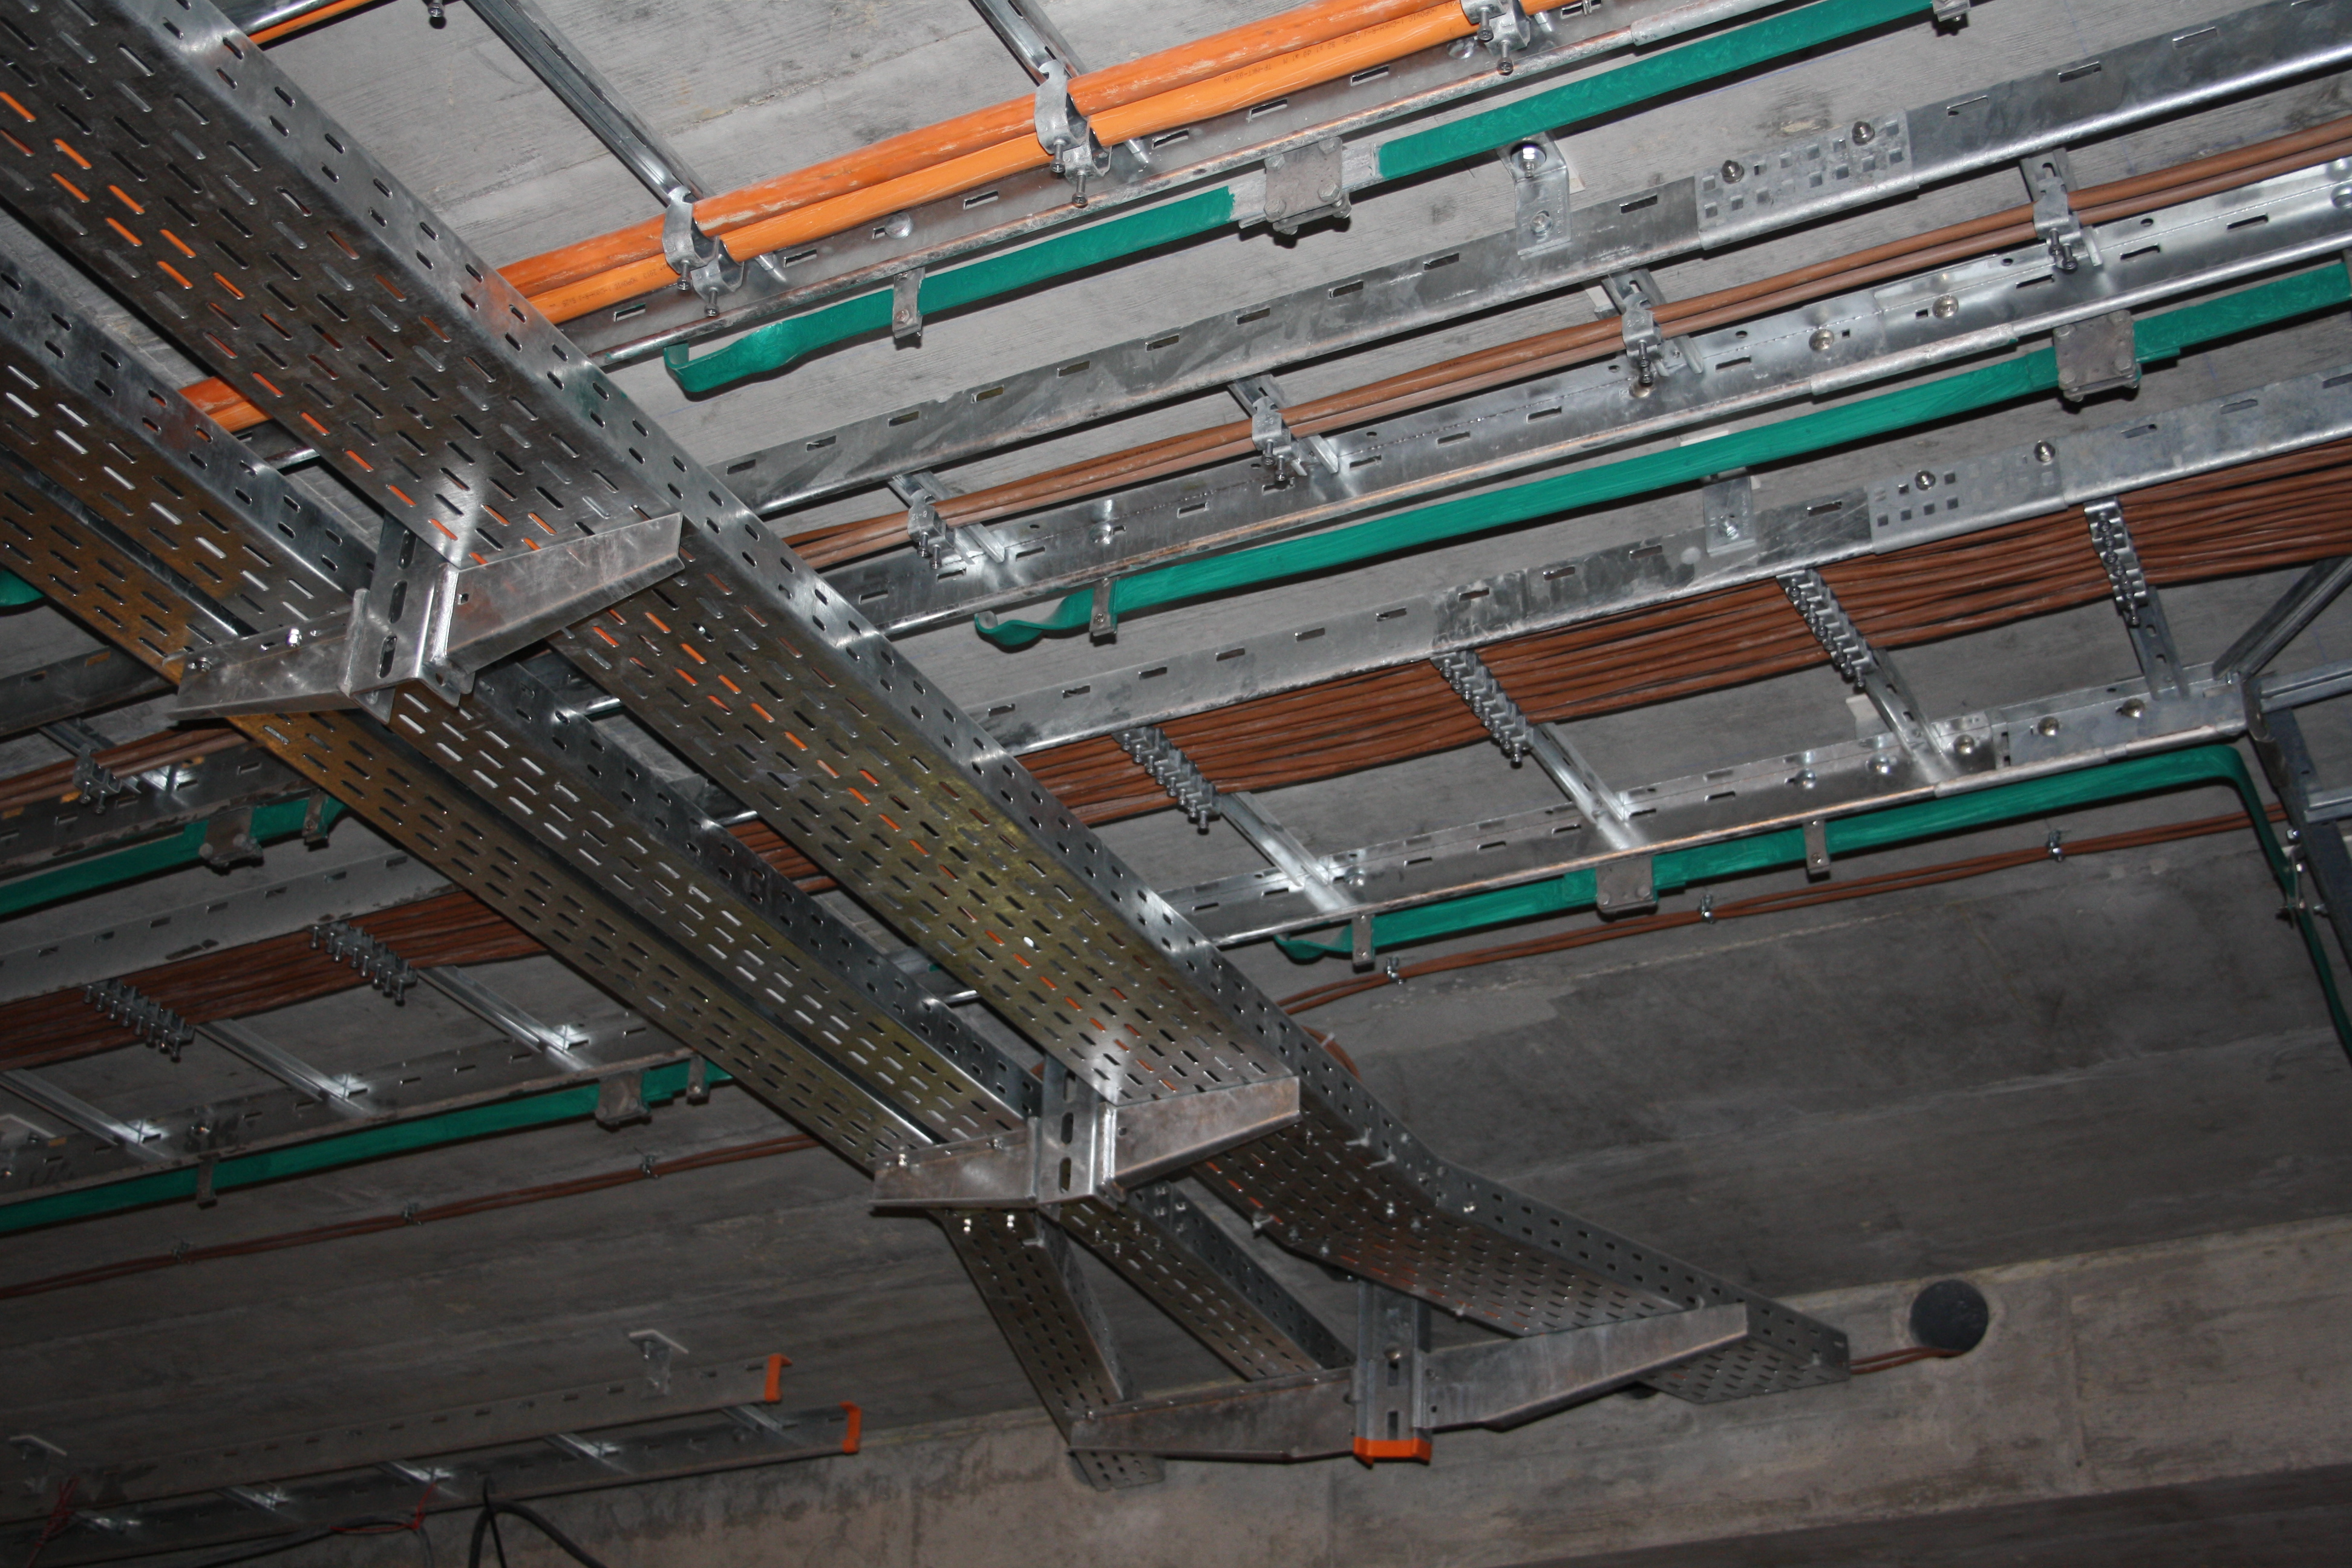
\includegraphics[width=0.47\textwidth]{elektryka/Cabtray_11.jpg} & % https://commons.wikimedia.org/wiki/File:Cabtray_11.jpg  Leotard, CC-0
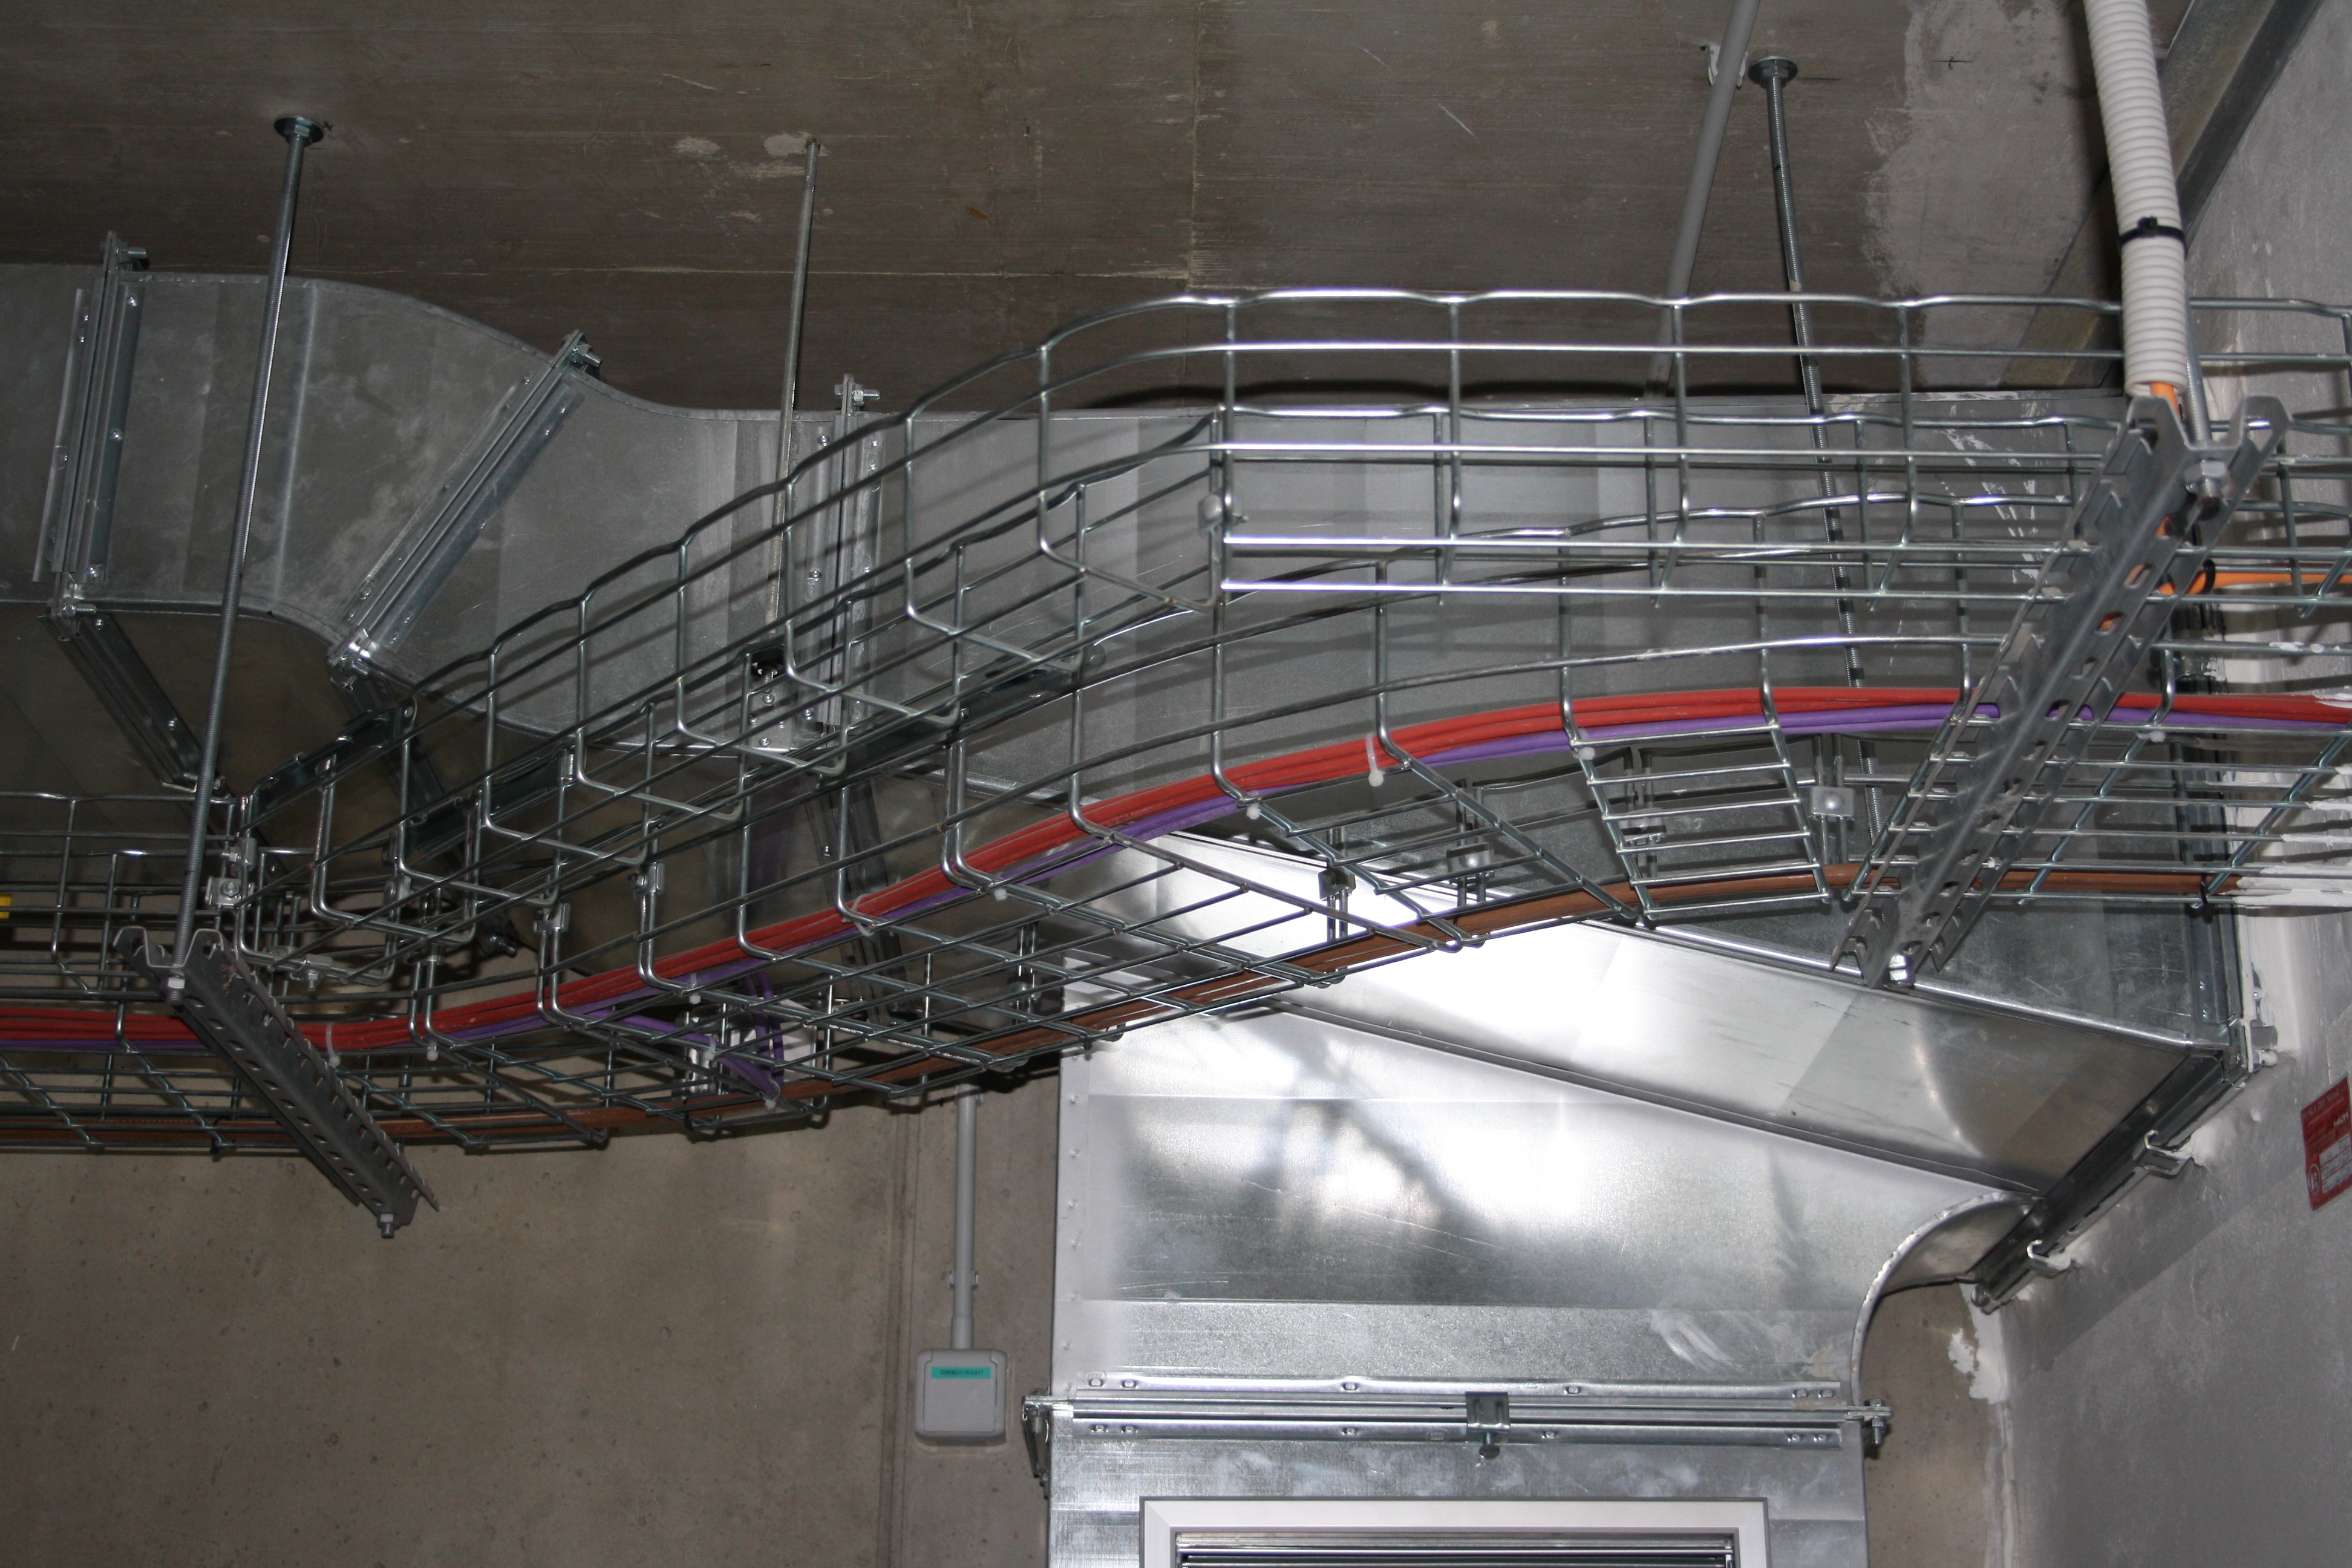
\includegraphics[width=0.47\textwidth]{elektryka/Cabtray_10.jpg} % https://commons.wikimedia.org/wiki/File:Cabtray_10.JPG  Leotard, CC-0
\\
koryta stalowe perforowane i drabiny kablowe &
koryta siatkowe
\end{tabular}\end{center}

\begin{center}\begin{tabular}{ccc}
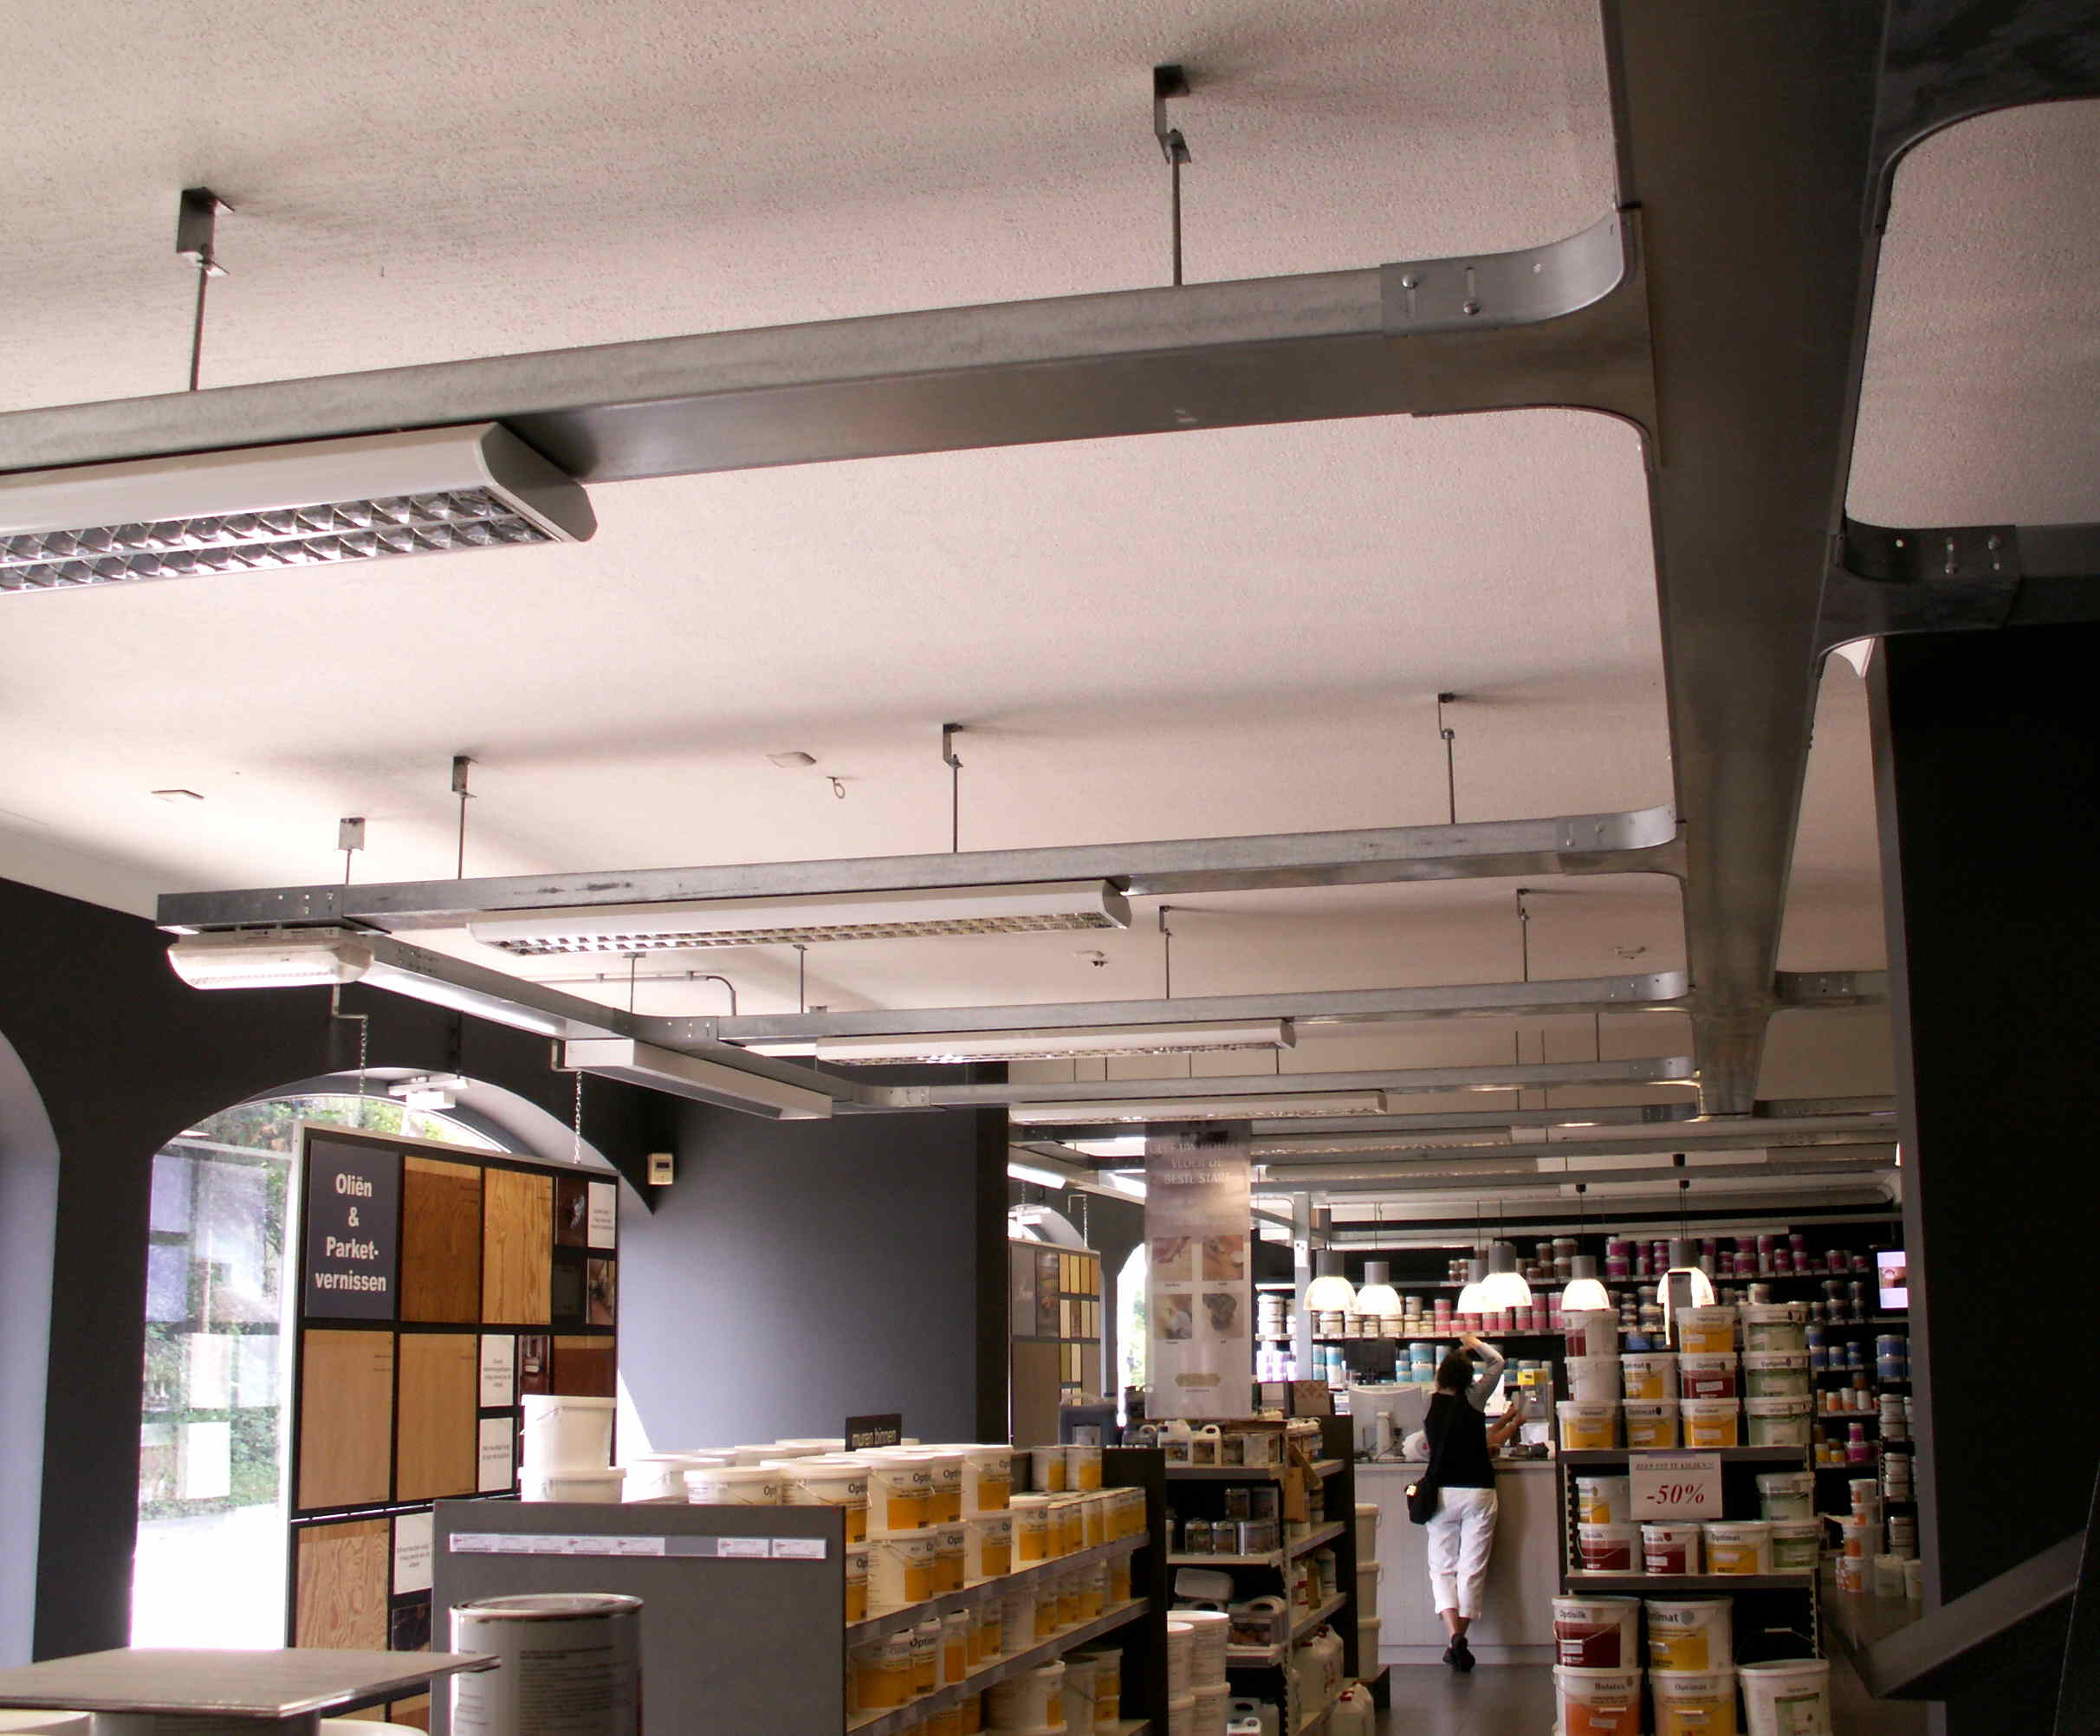
\includegraphics[trim={0 14cm 0 0},clip,width=0.47\textwidth]{elektryka/OrganizedElectricalWiring.jpg} & % https://commons.wikimedia.org/wiki/File:OrganizedElectricalWiring.jpg  KVDP, PD
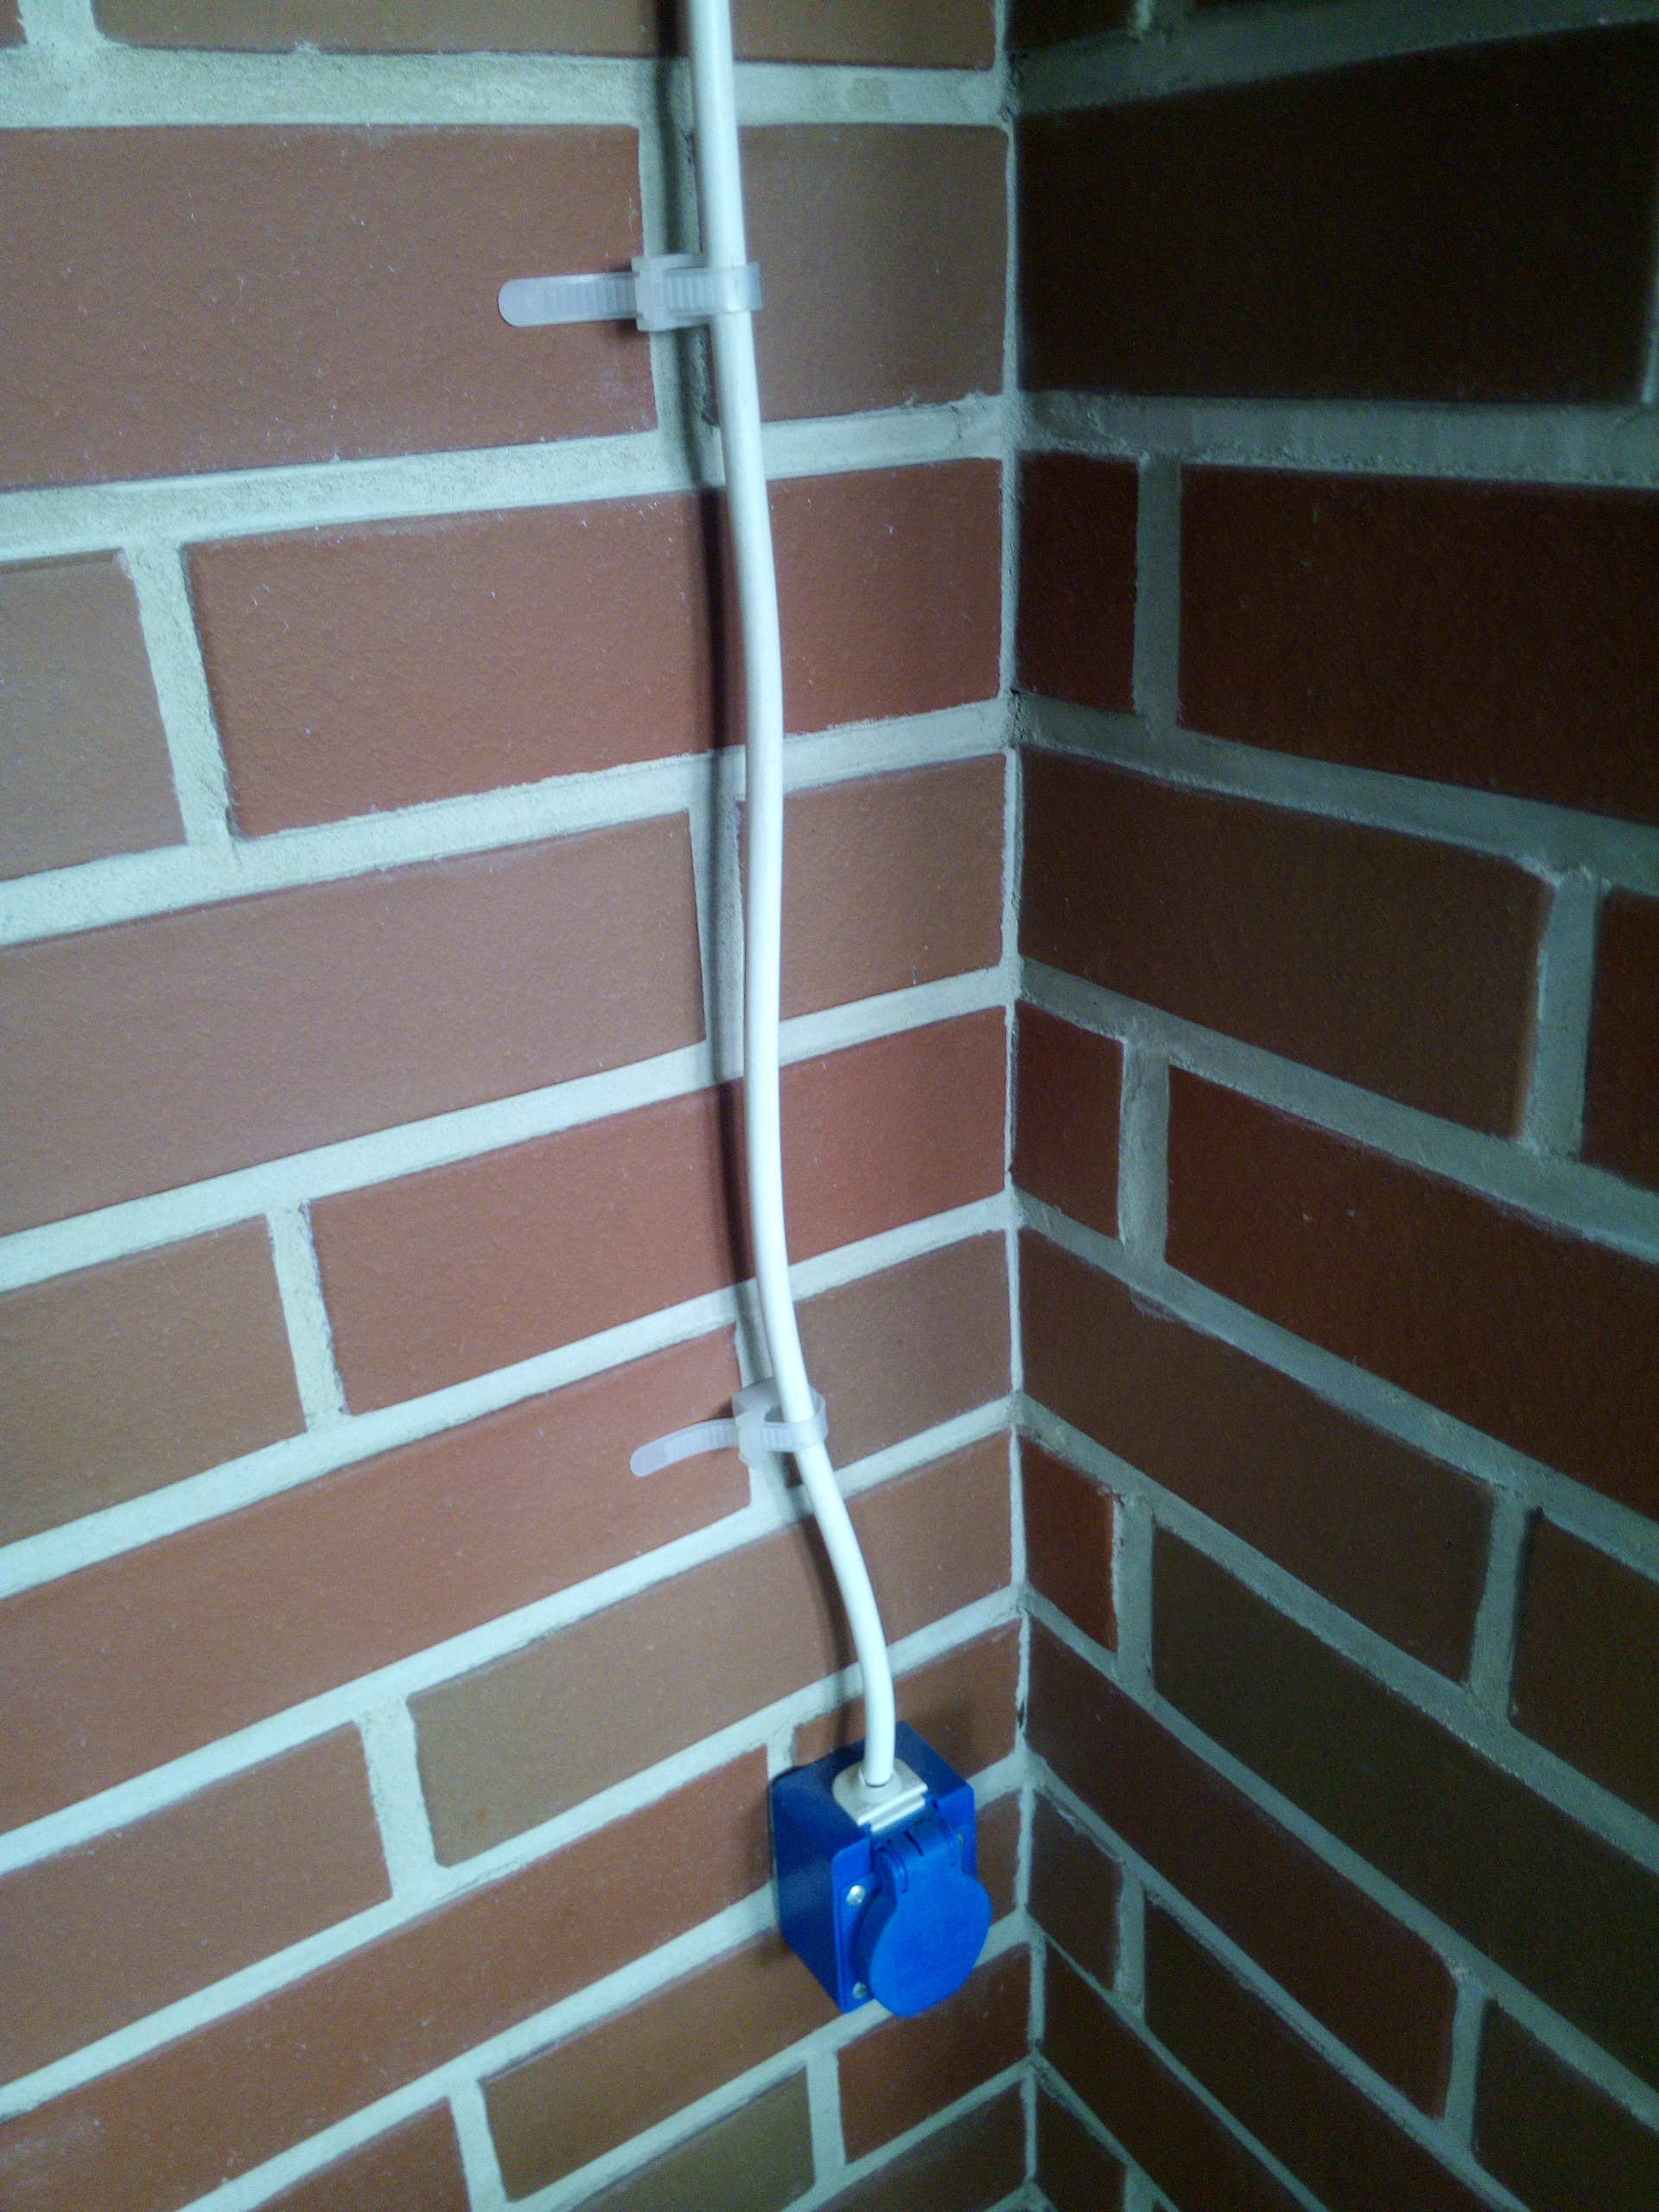
\includegraphics[trim={6cm 0 2cm 0},clip,width=0.176\textwidth]{elektryka/IMG_20210731_145157.jpg} &
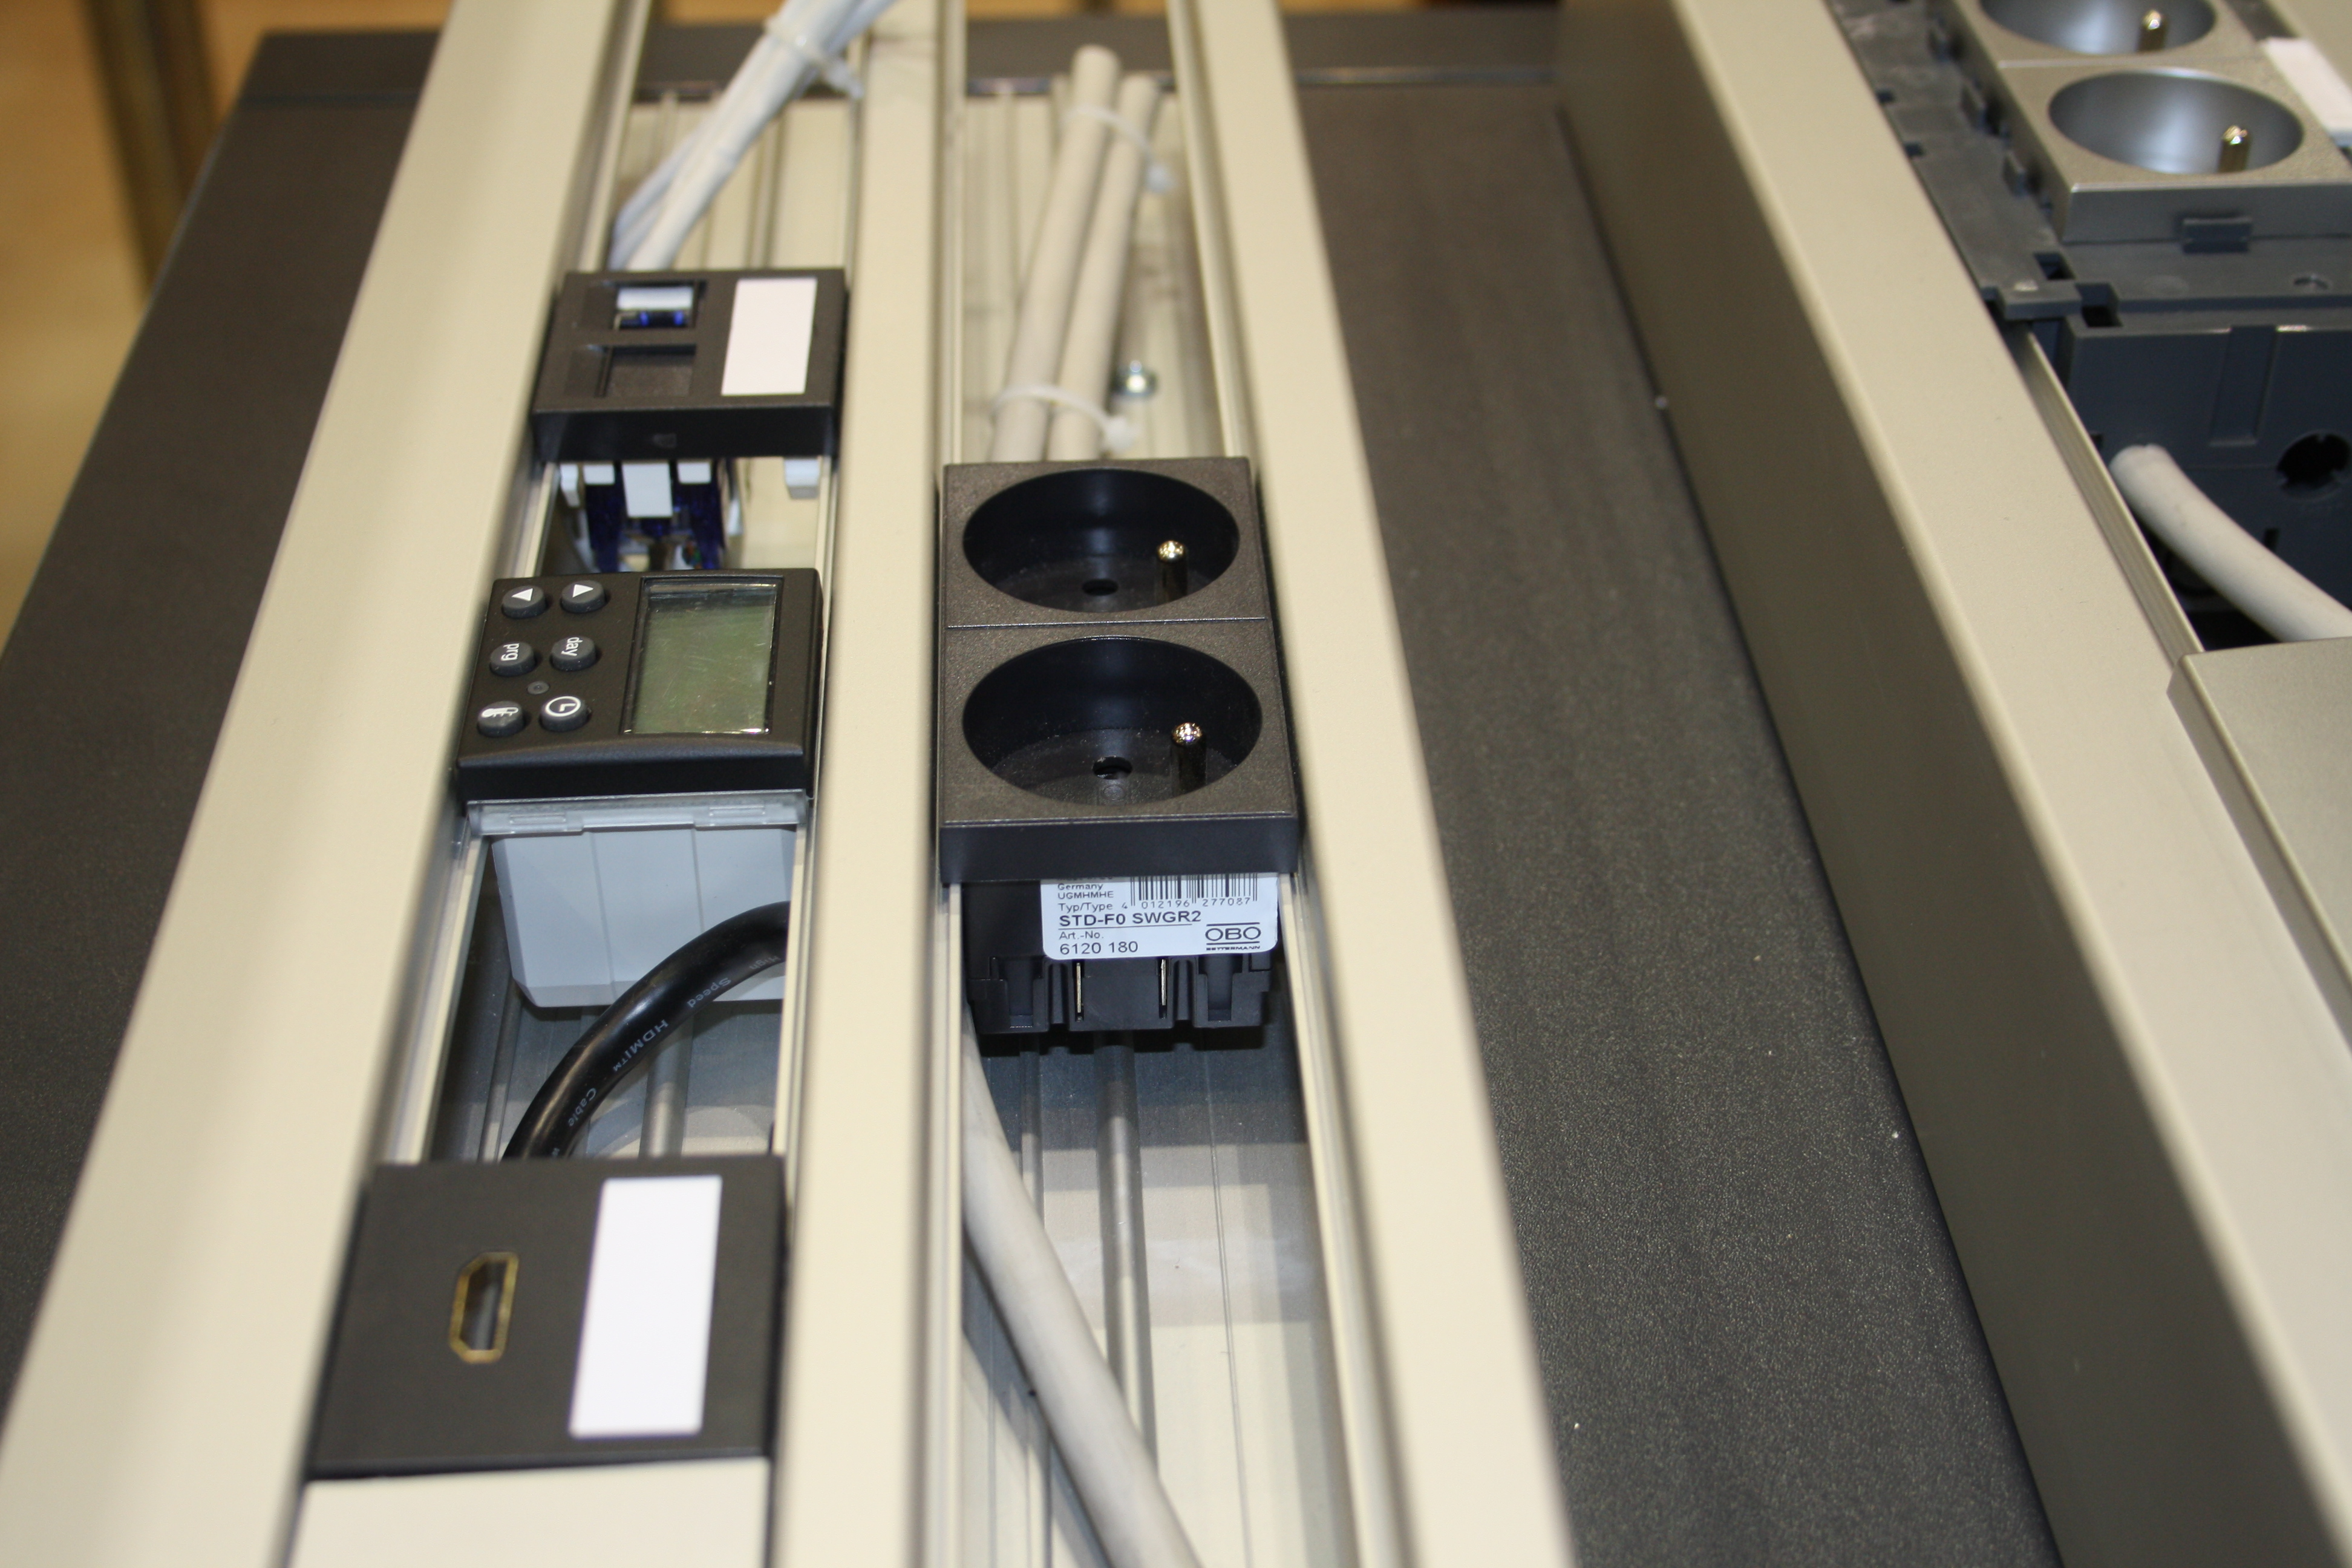
\includegraphics[trim={10cm 0 50cm 0},clip,width=0.263\textwidth]{elektryka/Cabtray_03.jpg} % https://commons.wikimedia.org/wiki/File:Cabtray_03.JPG  Leotard, CC-0
\\
koryta stalowe pełne &
instalacja natynkowa &
kanał instalacyjny PCV
\\
&
bez rurek &
z osprzętem 45x45mm
\end{tabular}\end{center}

\begin{center}\begin{tabular}{cc}
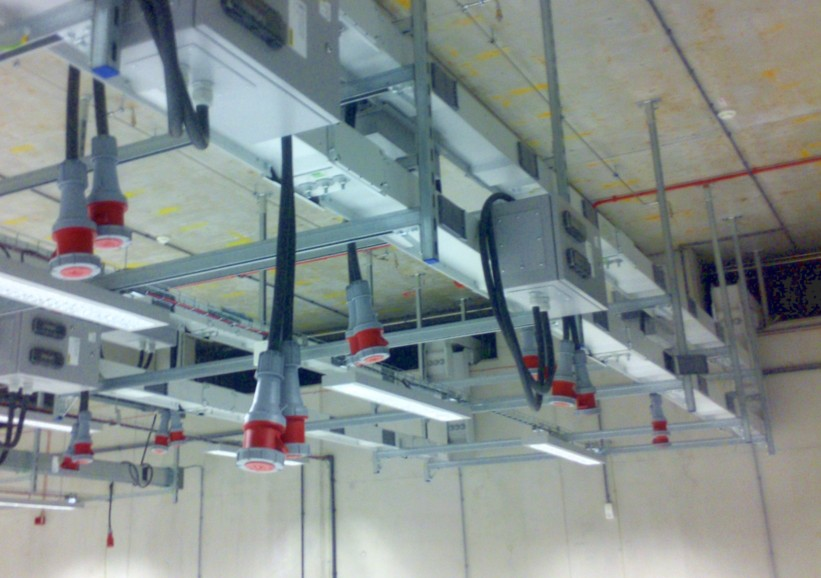
\includegraphics[width=0.47\textwidth]{elektryka/szynoprzewody.jpg} &
\\
szynoprzewody z kasetami dystrybucyjnymi &
\\
powieszone na konstrukcji z ceowników montażowych &
\end{tabular}\end{center}
\end{figure}

\subsubsection{montaż tras kablowych}

Elementy budujące „natynkowe” trasy kablowe, takie jak rurki, czy koryta mogą być montowane bezpośrednio do ściany.
Często jednak stosuje się dodatkowe konstrukcje służące ich zamocowaniu – zwłaszcza w przypadku koryt metalowych i szynoprzewodów.
Pozwalają one na montaż koryta do ściany lub sufitu z zachowaniem „orientacji” koryta w przestrzeni,
	czyli bez jego obracania, tak aby kable leżały na jego dnie a nie boku (dzięki czemu nie będą wypadać i nie ma potrzeby stosowania np. pokrywy do koryta).
Koryta mogą być mocowane do ścian przy użyciu różnego rodzaju wsporników, podwieszane do sufitu za pomocą szpilek,
	czy też montowane zarówno do ścian jak i sufitów na bardziej rozbudowanych konstrukcjach głównie z ceowników montażowych\footnote{
		Ceownik montażowy jest to profil (zazwyczaj stalowy) przypominający w przekroju literę C / U, gdzie boczne ścianki sa lekko zagięte do środka.
		Takie ukształtowanie zapewnia większą sztywność oraz pozwala na montaż elementów do „wnętrza” ceownika z użyciem nakrętek rombowych.
	}.
Zaletą zastosowania konstrukcji z ceowników w stosunku co do podwieszenia na szpilkach jest zapewnienie większej sztywności całej trasie kablowej.
Jest to szczególnie istotne przy montażu szynoprzewodów, które będą obciążane jeszcze dodatkowo skrzynkami odpływowymi –
	zwykłe ich podwieszenie na szpilach nie zapewni sztywności i pozornie sztywne szynoprzeody zaczną się skręcać i chwiać.

\begin{figure}[ht!]
\begin{center}\begin{tabular}{ccc}
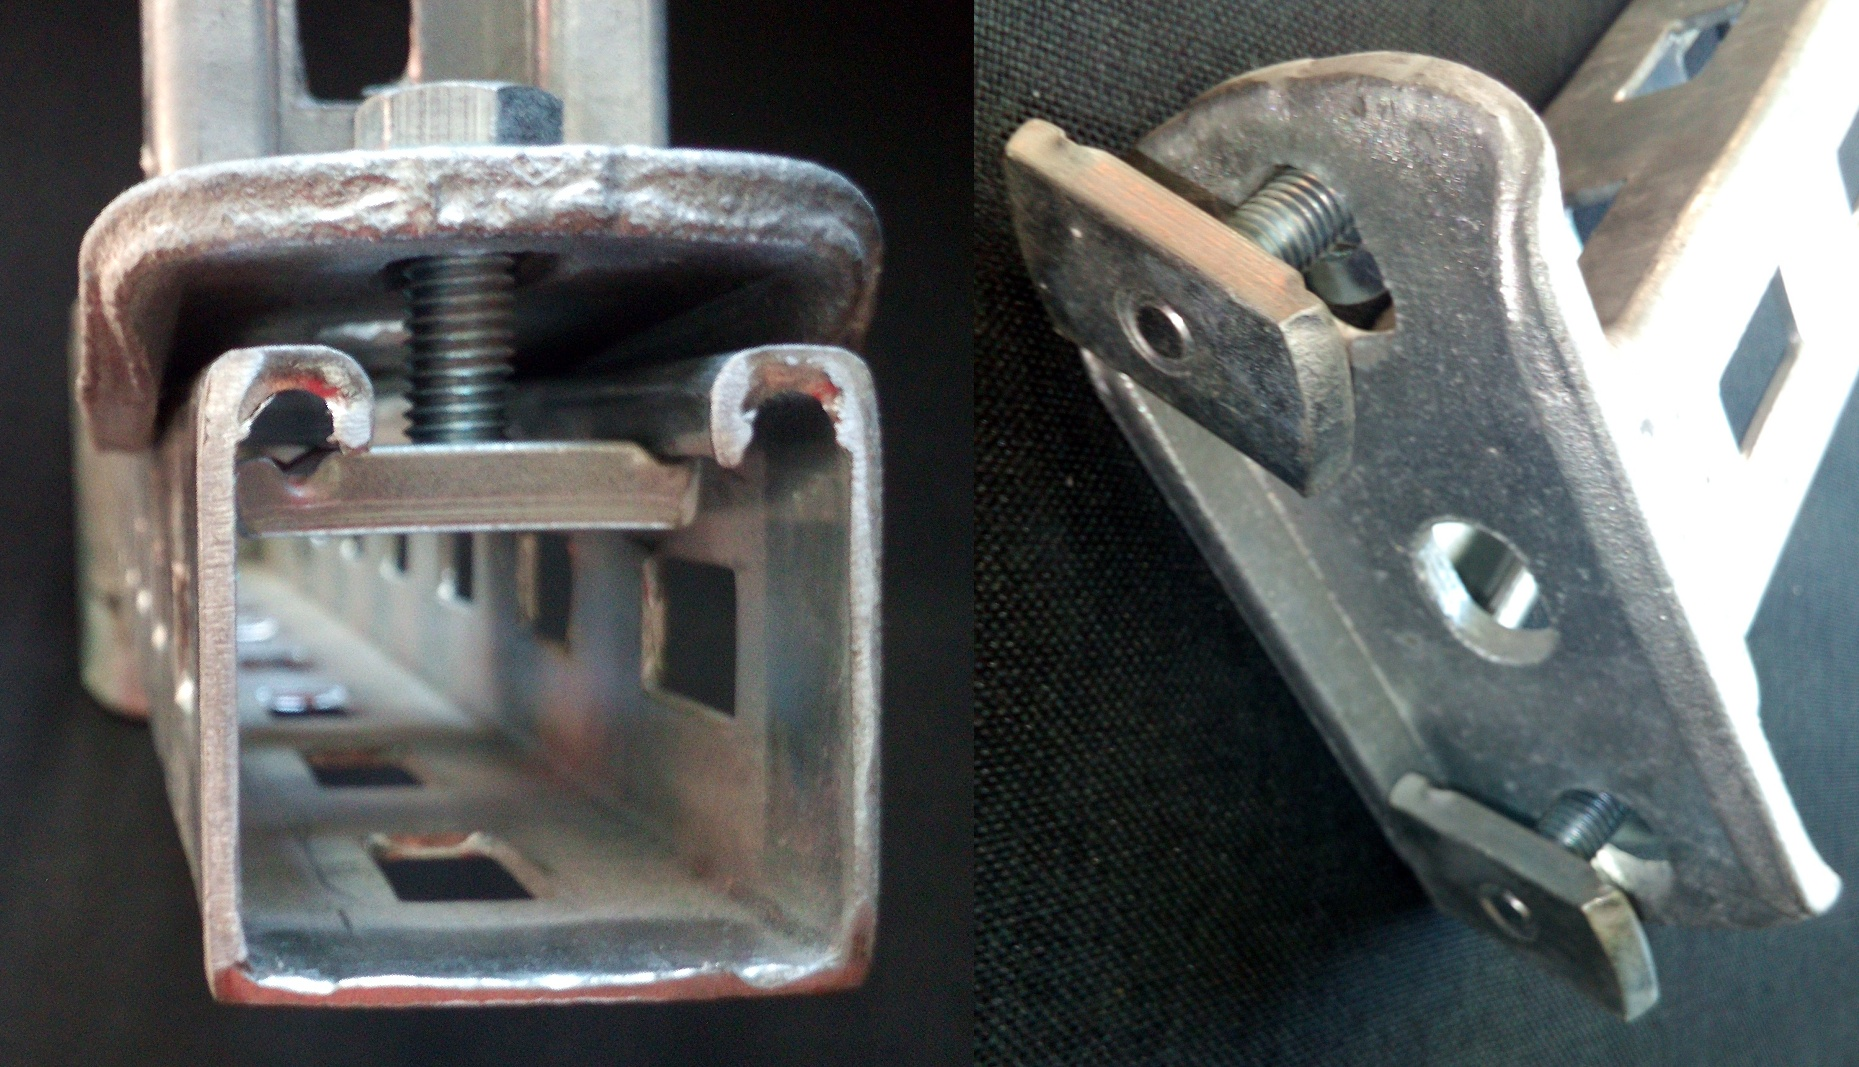
\includegraphics[height=5.5cm]{elektryka/ceowniki1.jpg} &
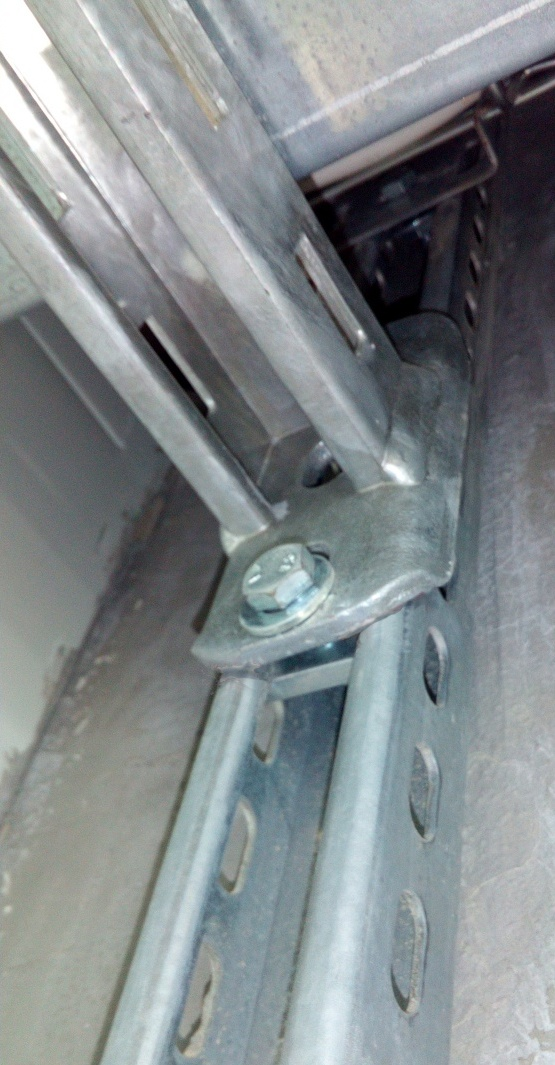
\includegraphics[height=5.5cm]{elektryka/ceowniki2.jpg} &
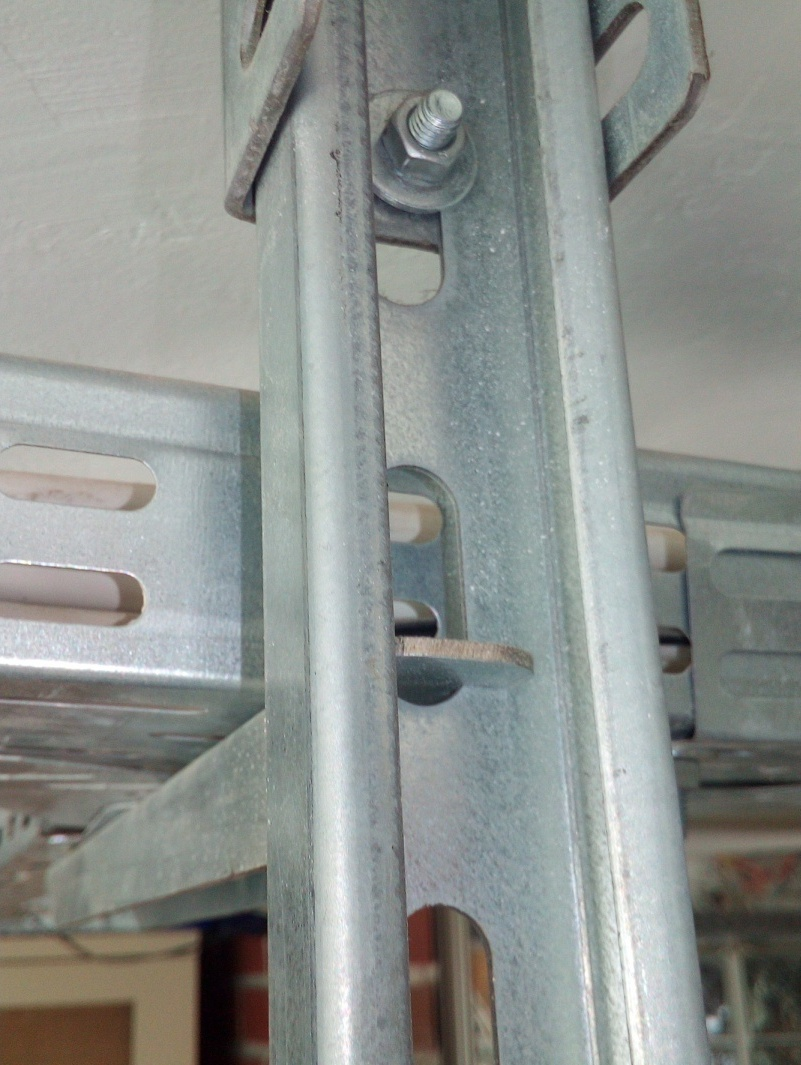
\includegraphics[height=5.5cm]{elektryka/ceowniki3.jpg}
\\
ceownik montażowy wraz z elementem &
wspornik zamocowany &
wykorzystanie perforacji 
\\
montowanym z użyciem nakrętki rombowej &
do ceownika &
ceownika do montażu
\end{tabular}\end{center}
\end{figure}

\subsection{rozdzielnice}

Przy planowaniu, projektowaniu rozdzielnic najistotniejsze jest zapewnienie odpowiednio dużo miejsca w rozdzielnicy – zarówno dla zmieszczenia samej aparatury i okablowania, jak też komfortu wykonywania prac serwisowych (dostęp do wszystkich elementów, zacisków, itd) oraz ew. rozbudowy czy modyfikacji. Przy wykonywaniu (prefabrykacji, montażu, kablowaniu) rozdzielnicy istotna jest estetyka i przejrzystość, która ułatwia późniejsze prace serwisowe.

Istnieje wiele rozwiązań konstrukcyjnych dla rozdzielnic elektrycznych, często nawet pojedynczy producent posiada kilka (niekompatybilnych ze sobą) takich systemów.
Konkretne rozwiązanie konstrukcyjne powinno być dobrane z uwzględnieniem tego co w danej rozdzielnicy będzie się znajdować i jak jest to montowane (szyna DIN, płyta montażowa, rack 19", ...).
Warto jednak pamiętać że na ogół nie wszystko musi się znaleźć w jednej obudowie i czasami lepiej jest zastosować osobną rozdzielnicę modułową i np. osobną obudowę z płytą montażową na pojedynczy duży aparat.
Albo osobną rozdzielnicę elektryczną i osobną szafkę rack na montaż kilku paneli krosowych i switcha.
Istotne jest dobre wykorzystanie miejsca i wykonanie zapewniające wygodę obsługi i serwisu.
Warto aby rozdzielnica zapewniała odpowiednią głębokość, ale raczej należy unikać montażu na kilku głębokościach na tej samej wysokości (pozwala to zmieścić więcej urządzeń, ale utrudnia dostęp).

\subsection{standardy}

\subsubsection{szyna DIN}

\begin{wrapfigure}{r}{2.7cm} %
\vspace{-0.8cm}\includegraphics[trim={0cm 0 0.2cm 0},clip,width=2.5cm]{img/elektryka/DIN-rail-dimensions}\vspace{-0.5cm} % https://commons.wikimedia.org/wiki/File:DIN-rail-dimensions.svg  Markus Kuhn as Public Domain
\end{wrapfigure}

Standard szyny \href{https://en.wikipedia.org/wiki/DIN_rail}{montażowej DIN} określa kilka rodzajów szyn.
Najpopularniejszą z nich jest szyna TH-35, szyli szyna o szerokości 35mm z blachy o grubości 1mm, zagłębiona w środkowej części na szerokości 25mm o co 7.5 mm lub 15mm (zależnie od wariantu).

Sam standard szyny nie określa niczego więcej.
W ogólności kształt obudów montowanych na szynę DIN nie jest zestandaryzowany (spotykane sa np. obudowy o wysokości kilkunastu cm).

Natomiast jest określony kształt obudów aparatury modułowej montowanej na szynę DIN.
Typowy moduł nie przekracza 47mm głębokości od szyny TH do części zakrywanej panelem przednim obudowy, 70mm głębokości od szyny TH do frontu aparatu, który liczy 45 mm wysokości.
Zapewnia to że większość aparatury modułowej da się zainstalować nawet w płytkiej rozdzielnicy bez możliwości regulacji głębokości szyn.
Natomiast szerokość przypadająca na jeden biegun zasilania wynosi 17.5mm, co pozwala na stosowanie standardowych szyn łączeniowych do aparatów.

Typowo długość szyny (szerokość zamontowanych na niej urządzeń) określa się właśnie w modułach o szerokości 17.5mm (±0.5mm).\footnote{Stosowane są także urządzenia o szerokości mniejszej niż jeden moduł – np. styki pomocnicze, złączki kablowe.}
Przez to, że standardowy jednopolowy wyłącznik nadprądowy posiada właśnie szerokość 1 modułu, to ilość modułów daje pewne wyobrażenie o wielkości rozdzielnicy.


\subsubsection{rack 19"}

Standard \href{https://en.wikipedia.org/wiki/19-inch_rack}{rack 19"} wywodzi się z telekomunikacji i jest powszechnie stosowany w rozwiązaniach IT.
Bywa jednak stosowany w zastosowaniach elektrycznych.
Stosowane są moduły wysokości 3U wyposażone w szynę DIN TH-35 do montażu aparatury elektrycznej w ramie rack 19".
Stosowane są także adaptery do montażu (odpowiednio krótkich) urządzeń rack 19" w (dostatecznie szerokich) rozdzielnicach elektrycznych.

Standard rack 19" (\href{https://www.server-racks.com/eia-310.html}{EIA-310}) określa jedynie podstawowe parametry montażowe dla płyt czołowych:
\begin{itemize}
	\item wymiary poziome:
	\begin{itemize}
		\item odległość pomiędzy wewnętrznymi krawędziami szyn montażowych (maksymalną szerokość obudowy montowanego urządzenia): 17~3/4" (450mm)
		\item ogległość pomiędzy środkami otworów montażowych: 18~5/16" (465.1mm)
		\item szerokość płyty czołowej urządzenia obejmującą otwory montażowe: 19" (482.6mm)
	\end{itemize}
\end{itemize}

~\vspace{-32pt}
\begin{wrapfigure}{r}{5.5cm}%
\vspace{-0.4cm}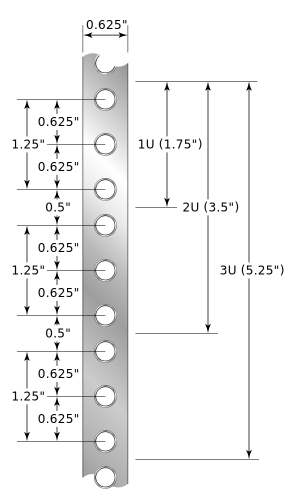
\includegraphics[width=5.3cm]{img/elektryka/Server_rack_rail_dimensions}\vspace{-2.6cm} % https://commons.wikimedia.org/wiki/File:Server_rack_rail_dimensions.svg  Sakurambo as Public Domain
\end{wrapfigure}

\begin{itemize}
	\item wymiary pionowe:
	\begin{itemize}
		\item jednostkę wysokości urządzenia \strong{\href{https://en.wikipedia.org/wiki/Rack_unit}{1U}}=1 3/4" (44.45mm)
		\item odległości środków trzech otworów montażowych w ramach każdego „U”:
			\begin{itemize}
				\item pierwszy otwór: 1/4" (6.35mm) od krawędzi
				\item środkowy otwór: 5/8" (7.95mm) od środka pierwszego
				\item trzeci otwór: 5/8" (7.95mm) od środka środkowego i 1/4" (6.35mm) od krawędzi
			\end{itemize}
			co razem daje 1 3/4" czyli jednostkę wysokości
	\end{itemize}
\end{itemize}

Standard pozwala także na stosowanie różnego typu otworów w profilu montażowym – gwintowane (3/16", 7/32", M5, lub M6), okrągłe niegwintowane lub kwadratowe (3/8" x 3/8", pozwalające na montaż nakrętki typu \textit{\href{https://www.server-racks.com/what-is-a-cagenut.html}{cage nut}}).

Natomiast nie określa:
\begin{itemize}
	\item głębokość szafy ani montowanego sprzętu
	\item formy ani sposobu mocowania jakichkolwiek dodatkowych podparć (dla długich urządzeń), prowadnic kulkowych, itp.
	\item \href{https://www.server-racks.com/rack-upright-shape.html}{kształtu profili} z otworami montażowymi
	\item ilości profili montażowych (czy występują środkowe / tylne)
	\item jakichkolwiek innych aspektów konstrukcyjnych szafy / stojaka (także tego czy to ma być zamknięta szafa czy w pełni otwarty stojak)
\end{itemize}

Można spotkać się także z odmianą 10" oraz 9.5" (half-rack). Ta druga pozwala na montaż dwóch urządzeń obok siebie w standardowym racku 19".


\copyrightFooter{
	© Robert Ryszard Paciorek <rrp@opcode.eu.org>, 2021.\\
	Wykorzystano grafiki należące do domeny publicznej.\\
	Kopiowanie, modyfikowanie i redystrybucja dozwolone pod warunkiem zachowania informacji o autorach.
}
\end{document}
